\documentclass[12pt,twoside]{article}
\usepackage{indentfirst}
\usepackage[nottoc,notlof,notlot]{tocbibind}
\usepackage{fancyhdr,ragged2e}
\usepackage{todonotes}
\fancyhead{}
%%%%%%%%%%%%%%%%%%%%%%%%%%%%%%%%%%%%%%%%%%%%%%%%%%%%%%%%%%%%%%%%%%%%%%%%%%%%%

% Definitions for the title page
% Edit these to provide the correct information
% e.g. \newcommand{\reportauthor}{Timothy Kimber}

\newcommand{\reporttitle}{Evaluating the Use of Machine Learning for Doubly-Robust Estimation in Missing Data}
\newcommand{\reportauthor}{Juliette Maïko Limozin}
\newcommand{\supervisor}{Dr David Whitney}
\newcommand{\degreetype}{Mathematics}
\newcommand{\expit}{\text{expit}}
%%%%%%%%%%%%%%%%%%%%%%%%%%%%%%%%%%%%%%%%%%%%%%%%%%%%%%%%%%%%%%%%%%%%%%%%%%%%%

% load some definitions and default packages
%%%%%%%%%%%%%%%%%%%%%%%%%%%%%%%%%%%%%%%%%
% University Assignment Title Page 
% LaTeX Template
% Version 1.0 (27/12/12)
%
% This template has been downloaded from:
% http://www.LaTeXTemplates.com
%
% Original author:
% WikiBooks (http://en.wikibooks.org/wiki/LaTeX/Title_Creation)
%
% License:
% CC BY-NC-SA 3.0 (http://creativecommons.org/licenses/by-nc-sa/3.0/)
% 
%
%%%%%%%%%%%%%%%%%%%%%%%%%%%%%%%%%%%%%%%%%
%----------------------------------------------------------------------------------------
%	PACKAGES AND OTHER DOCUMENT CONFIGURATIONS
%----------------------------------------------------------------------------------------
\usepackage[a4paper,hmargin=2.5cm,vmargin=2.5cm,includeheadfoot]{geometry}
\usepackage{textpos}
\usepackage{natbib} % for bibliography
\usepackage{tabularx,longtable,multirow,subfigure,caption}%hangcaption
\usepackage{fncylab} %formatting of labels
\usepackage{fancyhdr} % page layout
\usepackage{url} % URLs
\usepackage[english]{babel}
\usepackage{amsmath}
\usepackage{graphicx}
\usepackage{dsfont}
\usepackage{epstopdf} % automatically replace .eps with .pdf in graphics
\usepackage{backref} % needed for citations
\usepackage{array}
\usepackage{latexsym}
\usepackage[pdftex,pagebackref,hypertexnames=false,colorlinks]{hyperref} % provide links in pdf

\hypersetup{pdftitle={},
  pdfsubject={}, 
  pdfauthor={},
  pdfkeywords={}, 
  pdfstartview=FitH,
  pdfpagemode={UseOutlines},% None, FullScreen, UseOutlines
  bookmarksnumbered=true, bookmarksopen=true, colorlinks,
    citecolor=black,%
    filecolor=black,%
    linkcolor=black,%
    urlcolor=black}

\usepackage[all]{hypcap}


%\usepackage{color}
%\usepackage[tight,ugly]{units}
%\usepackage{float}
%\usepackage{tcolorbox}
%\usepackage[colorinlistoftodos]{todonotes}
% \usepackage{ntheorem}
% \theoremstyle{break}
% \newtheorem{lemma}{Lemma}
% \newtheorem{theorem}{Theorem}
% \newtheorem{remark}{Remark}
% \newtheorem{definition}{Definition}
% \newtheorem{proof}{Proof}


%%% Default fonts
\renewcommand*{\rmdefault}{bch}
\renewcommand*{\ttdefault}{cmtt}



%%% Default settings (page layout)
\setlength{\parindent}{0em}  % indentation of paragraph

\setlength{\headheight}{14.5pt}

\fancyfoot[ER,OL]{\sffamily\textbf{\thepage}}%Page no. in the left on odd pages and on right on even pages
\fancyfoot[OC,EC]{\sffamily }
\renewcommand{\headrulewidth}{0.1pt}
\renewcommand{\footrulewidth}{0.1pt}
\captionsetup{margin=10pt,font=small,labelfont=bf}


%--- chapter heading

\def\@makechapterhead#1{%
  \vspace*{10\p@}%
  {\parindent \z@ \raggedright \sffamily
    \interlinepenalty\@M
    \Huge\bfseries \thechapter \space\space #1\par\nobreak
    \vskip 30\p@
  }}

%---chapter heading for \chapter*  
\def\@makeschapterhead#1{%
  \vspace*{10\p@}%
  {\parindent \z@ \raggedright
    \sffamily
    \interlinepenalty\@M
    \Huge \bfseries  #1\par\nobreak
    \vskip 30\p@
  }}

\allowdisplaybreaks

% load some macros
% Here, you can define your own macros. Some examples are given below.

\newcommand{\R}[0]{\mathds{R}} % real numbers
\newcommand{\Z}[0]{\mathds{Z}} % integers
\newcommand{\N}[0]{\mathds{N}} % natural numbers
\newcommand{\C}[0]{\mathds{C}} % complex numbers
\renewcommand{\vec}[1]{{\boldsymbol{{#1}}}} % vector
\newcommand{\mat}[1]{{\boldsymbol{{#1}}}} % matrix


\date{June 2021}

\begin{document}

% load title page
% Last modification: 2015-08-17 (Marc Deisenroth)
\begin{titlepage}

\newcommand{\HRule}{\rule{\linewidth}{0.5mm}} % Defines a new command for the horizontal lines, change thickness here


%----------------------------------------------------------------------------------------
%	LOGO SECTION
%----------------------------------------------------------------------------------------


\includegraphics[width = 4cm]{./figures/imperial}\\[0.5cm] 

\center % Center remainder of the page

%----------------------------------------------------------------------------------------
%	HEADING SECTIONS
%----------------------------------------------------------------------------------------

\textsc{\Large Imperial College London}\\[0.5cm] 
\textsc{\large Department of Mathematics}\\[0.5cm] 

%----------------------------------------------------------------------------------------
%	TITLE SECTION
%----------------------------------------------------------------------------------------

\HRule \\[0.4cm]
{ \huge \bfseries \reporttitle}\\ % Title of your document
\HRule \\[1.5cm]
 
%----------------------------------------------------------------------------------------
%	AUTHOR SECTION
%----------------------------------------------------------------------------------------

\begin{minipage}{0.4\textwidth}
\begin{flushleft} \large
\emph{Author:}\\
\reportauthor % Your name
\end{flushleft}
\end{minipage}
~
\begin{minipage}{0.4\textwidth}
\begin{flushright} \large
\emph{Supervisor:} \\
\supervisor % Supervisor's Name
\end{flushright}
\end{minipage}\\[4cm]


%----------------------------------------------------------------------------------------
%	FOOTER & DATE SECTION
%----------------------------------------------------------------------------------------
\vfill % Fill the rest of the page with whitespace
Submitted in partial fulfillment of the requirements for the MSci degree in
\degreetype~of Imperial College London\\[0.5cm]

\makeatletter
\@date 
\makeatother


\end{titlepage}



% page numbering etc.
\pagenumbering{roman}
\clearpage{\pagestyle{empty}\cleardoublepage}
\setcounter{page}{1}
\pagestyle{fancy}
\setlength{\parindent}{5ex}
%%%%%%%%%%%%%%%%%%%%%%%%%%%%%%%%%%%%
\begin{abstract}

Doubly-robust estimation is a popular method for estimating the outcome mean of a data set missing outcome values at random. This estimator is based on predictive models of the outcome distribution and the propensity score. If at least one of these models is correctly specified, the doubly-robust estimator is consistent for the true outcome mean. Traditionally, parametric methods of model specification are preferred but often lead to misspecification. We illustrate the use of nonparametric Machine Learning tools for nuisance parameter model setting, specifically Random Forests and Multi-Layer Perceptrons. In the simulations we ran on specific data sets, we empirically found that these methods often provide $N^{-1/2}$-consistent doubly-robust estimators and hence provide more degrees of freedom for correct model specification, even though popular 'off the shelf' methods for choosing the learning hyperparameters of these Machine Learning algorithms failed to provide confidence interval construction with nominal coverage, and bias convergence rates could be further improved. The findings in this report highlight the potential of Machine Learning approaches for improving the performance and robustness of doubly-robust estimation, but also the need for a deeper understanding and study of model selection and hyperparameter tuning to achieve higher rates of convergence that would improve DR estimation performance in a nonparametric setting.

\end{abstract}

\clearpage
%%%%%%%%%%%%%%%%%%%%%%%%%%%%%%%%%%%%
\section*{Acknowledgments}
I would like to thank my project supervisor, Dr David Whitney, for his continued guidance and support throughout this project. Our weekly meetings have always been a pleasure, and his advice on postgraduate studies have also been of immense help. 

I would also like to thank my family, who even though might not understand Statistics at a Master's level, have always enabled me to achieve my best.

Last but not least, I would like to thank my various statistics lecturers who, in my 4 years at Imperial, have enamoured me with their passion for Statistics.

\clearpage{\pagestyle{empty}\cleardoublepage}

%%%%%%%%%%%%%%%%%%%%%%%%%%%%%%%%%%%%
%--- table of contents
\tableofcontents 

\clearpage
\listoffigures
\listoftables

\clearpage
\pagenumbering{arabic}
\setcounter{page}{1}
\fancyhead[L]{\textsl{\leftmark}}

\setcitestyle{authoryear,open={(},close={)}}
%%%%%%%%%%%%%%%%%%%%%%%%%%%%%%%%%%%%
\section{Introduction} 

Missing data is a common issue encountered in Statistics, and can have a significant effect on statistical inferences one may draw from this type of data. Suppose one wishes to estimate the mean outcome value of a data set that has some missing outcome values. One way to approach this issue is to simply discard the data points for which we do not have an outcome value accounted, but that would lead to a loss of valuable feature information we still have of these data points, and this estimation would likely be biased.

Many bias-minimising strategies exist for estimating the mean outcome value. The most efficient method consists of fitting predictive models of the nuisance parameters, i.e. the outcome distribution and the probability of observing the outcome given the feature data (referred to as propensity score), and using the fitted values as part of the outcome mean calculation. Such a way of estimating the outcome mean is called the augmented inverse probability weighting (AIPW) approach, often referred to as doubly-robust (DR) estimation. This approach has been popularised in many fields, as it provides the user two chances of maintaining consistency, as only one of the two predictive models needs to be correctly specified. The art of specifying these models, however, is the biggest challenge one has to face when using DR estimation. We wish to consider models of the nuisance parameters that are not only accurate but also provide a DR estimate whose bias converges to 0 at a rate faster than that of $N^{-1/2}$ ($N$ being the sample size), which is generally the rate of convergence to the true value that we aim for in statistical literature.

Traditionally, parametric models are used to predict the outcome and the propensity score. As parametric models form a family of probability distributions, their parameter range is finite and they provide useful theoretical backings such as the ability to infer asymptotic distributions and confidence intervals (CIs). However, slight misspecification can lead to biased estimates. In recent years, developments in data-adaptive non-parametric tools have made Machine Learning (ML) approaches more attractive in the model setting. The main question we wish to answer in this report is whether these ML tools provide an advantage over the parametric methods for correctly specifying nuisance parameter models in DR estimation, whilst maintaining low bias and nominal CI coverage.
 
In this report we will illustrate the use of DR estimation, starting with a parametric setting that includes DR estimates with one or more misspecified models. We will then move towards flexible nonparametric methods, notably Random Forests (RFs) and Multilayer Perceptrons (MLPs), to identify if they provide improved inference while still maintaining consistent estimation. As we shall demonstrate in section 3, parametric models are likely to be misspecified in practice and the misspecification leads to highly biased estimators with CIs not containing the true value as sample sizes increase. In section 4, we suggest that flexible nonparametric methods such as RFs and MLPs give good DR estimator bias performance as they provide more degrees of freedom to get a correct specification of the nuisance parameter models. However they have difficulty reaching a high convergence rate of the bias, and CIs constructed using nuisance parameter models-based SE estimation as suggested by \cite{davidian} also lead non-optimal rate of convergence to high coverage. \cite{benkeser2017} have proposed alternative correction procedures to provide DR estimators with almost-nominal CI coverage. However, the results presented in this report suggest that more research must be conducted on how to optimise hyperparameter tuning (the selection of the parameters of an ML model used to control its learning process) of such nonparametric methods to reduce DR estimation bias with higher convergence rate.


\section{Setting} 

Suppose we have a data set of sample size $N$, and realisations of random vector $(\mathbf{Y}, \mathbf{W}, \mathbf{R})$ where $\mathbf{Y}$ denotes a partially denoted outcome, i.e. $Y_i$ is missing for individual $i$'s unobserved outcome. $\mathbf{W}$ denotes the auxiliary variables, and $\mathbf{R}$ is an indicator on whether the $i$th individual's outcome is missing or not; that is, if $R_i = 1$, the outcome is observed, whereas $R_i = 0$ would indicate that the outcome is missing.
To summarise:
\begin{itemize}
    \item $\mathbf{Y}$: partially observed outcome 
    \item $\mathbf{W}$: auxiliary variables/covariates 
    \item $\mathbf{R}$: indicator on whether $Y$ is observed or not ($R = 1$: observed, $R = 0$: missing) 
\end{itemize}

The outcome is said to be \textbf{missing at random (MAR)} if the conditional probability that a particular missingness pattern occurs given the data is independent of the missing values in that pattern \citep{vansteelandt}, i.e $P(R=r|\mathbf{W}, Y) = P(R= r|\mathbf{W})$ and  $P(Y=y|\mathbf{W}, R) = P(Y=y|\mathbf{W})$. So in the example of a clinical trial, we would consider the data set obtained from the study to be MAR if, given the measurements taken from the patients, the reasons why some patients dropped out were unrelated to the outcome of the trial. The MAR setting will therefore have effects on any statistical inference we may perform on this data set.

When the missingness pattern is independent of both the auxiliary variables and the outcome data, the data set is said to be \textbf{missing completely at random (MCAR)}, i.e. $P(R=r|\mathbf{W}, Y) = P(R = r)$ and  $P(Y=y|\mathbf{W}, R) = P(Y=y)$. Hence any estimation on the outcome data is unbiased, but a data set is, in practice, rarely MCAR.\\

We make the assumption that $(\mathbf{W}_1, Y_1, R_1),...,(\mathbf{W}_N, Y_N, R_N)$ are independent and identically distributed for the rest of the report. We also assume that $R$ is independent of $Y$ given $\mathbf{W}$ so $(\mathbf{W}_1, Y_1, R_1), ... ,(\mathbf{W}_N, Y_N, R_N)$ are MAR \citep{vansteelandt}, where the index $i = 1,...,N$ denotes the $i$th individual of the data.\\

\section{Non-robust and DR estimators}

\subsection{Inverse Probability Weighting approach}

Suppose we wish to calculate or estimate the outcome mean $\beta = E(\mathbf{Y})$. A problem occurs when trying to compute it as $\mathbf{Y}$ is only partially observed, so calculating an estimate of the outcome mean with only the observed outcomes values would be a biased estimation in a MAR setting.

One solution to this problem is the inverse probability weighting (IPW) approach. Its name comes from the fact that each observed outcome $Y_i$ (called \textit{complete} case) is weighted by the propensity score, denoted by
\begin{align*}
    \pi(\mathbf{W})= E(R|\mathbf{W}) = P(R = 1|\mathbf{W}).
\end{align*}

We assume that the weighting is bounded away from 0 almost for any $\mathbf{W}_i$.

The IPW estimator of the mean $\beta$ is then simply 
\begin{equation} \label{IPW_est}
    \hat{\beta}_{IPW} = \frac{1}{N} \sum_{i=1}^{N} \frac{R_iY_i}{\pi(\mathbf{W}_i)}.
\end{equation}

In practice, the propensity score $\pi(\mathbf{W})$ is unknown, so we predict the probabilities using, most commonly, a parametric model $\hat\pi(\mathbf{W}; \boldsymbol\alpha)$ for the missingness pattern and we build an estimator $\hat{\boldsymbol\alpha}$ of $\boldsymbol\alpha$ from the data \citep{vansteelandt}.

If the propensity score model $\hat\pi(\mathbf{W}; \boldsymbol\alpha)$ is correctly specified, by the weak law of large numbers (WLLN), $\hat{\beta}_{IPW}$ will converge in probability to the true mean $\beta$, so this makes the IPW estimate consistent for $\beta$ \citep{davidian}. Using the Central Limit Theorem (CLT), we have $\sqrt{N}(\hat{\beta}_{IPW}-\beta) \xrightarrow{d} \mathcal{N}(0,\sigma^2)$. In practice since we do not know $\sigma^2$ we use the estimated outcome variance $\hat\sigma$ (often a sample-based estimator), to be able to perform inference tests and CIs for the true mean.

A drawback from the IPW estimator in equation \ref{IPW_est} is that it is usually difficult to construct a propensity score model unless the auxiliary variables $\mathbf{W}$ are categorical or the sample size $N$ is large enough, so removal of bias is not guaranteed by the IPW estimator when the model is misspecified. Another problem that arises is unstable weights: due to practical positivity violations, the fitted probability of observing an outcome given the auxiliary variables may be very small for the majority of individuals, and very large for a small subgroup of the sample data that has rarely been observed, so the IPW estimator is mainly dominated by these large weights \citep{seaman}. \cite{petersen} have proposed various methods for responding to practical positivity violations, notably for inference based on the IPW approach.

\citet{kang} suggest that the model being misspecified is more likely the cause of large weights, rather than if the auxiliary variables are truly predictive of whether the outcome may be missing or not. There exist a few tests, including the \citet{hosmer} test, to detect poor fit of the propensity score model.\\

\subsection{Regression imputation approach} 

Alternatively, one could make use of the conditional expectation of the outcome 
\begin{align*}
    m(\mathbf{W}) = E(Y|R= 1,\mathbf{W})
\end{align*}
to have a different estimator of the mean \citep{davidian,vansteelandt}, sometimes called the regression imputation estimator: 

\begin{equation}
    \hat{\beta}_ {RI} = \frac{1}{N}\sum_{i=1}^N m(\mathbf{W}_i)
\end{equation}

In practice the true value of $m(\mathbf{W})$ is unknown, we propose an outcome model, most commonly a parametric model $\hat m(\mathbf{W}, \gamma)$ with some parameter $\gamma$, and again we build an estimator $\hat{\gamma}$ for $\gamma$ from the sample data. Like in IPW, the efficiency of the RI estimator in terms of consistency relies on the correct specification of the outcome model, as then the WLLN would apply and so the RI estimator would be consistent for $\beta$. \\

\subsection{Augmented IPW approach} 

The estimation strategies from the previous sections motivate the idea behind the AIPW estimator. One could think of combining the ideas from the IPW and RI estimators. From \citet{davidian}, IPW estimators of $\beta$, when the propensity score model is correctly specified and the estimators are consistent and are asymptotically normal (i.e. CLT holds), are equivalent to 

\begin{equation}
    \frac{1}{N}\sum_{i=1}^{N}\frac{R_iY_i}{\hat\pi(\mathbf{W}_i, \hat{\alpha})} - \frac{1}{N}\sum_{i=1}^{N} \left(1 - \frac{R_i}{\hat\pi(\mathbf{W_i},\hat{\alpha})} \right) h(\mathbf{W}_i)
\end{equation}

This is called an AIPW as it is the sum of the IPW estimator and an augmentation term depending on $h(\mathbf{W})$ \citep{davidian}. By taking $-h(\mathbf{W}) = \hat m(\mathbf{W}, \hat{\gamma})$ like in the RI approach, we have a new estimator
\begin{equation}
    \hat\beta_{DR} = \frac{1}{N}\sum_{i=1}^{N}\frac{R_iY_i}{\hat \pi(\mathbf{W}_i, \hat{\alpha})} + \frac{1}{N}\sum_{i=1}^{N} \left(1 - \frac{R_i}{\hat\pi(\mathbf{W_i},\hat{\alpha})} \right) \hat m(\mathbf{W}_i, \hat\gamma)
\end{equation}

The estimator $\hat\beta_{DR}$ is consistent (i.e $\hat\beta_{DR}$ converges in probability to the true mean $\beta$) and asymptotically normal when either the propensity score or outcome model are correctly specified, as the correct specification of one suffices for consistency, and therefore the CLT to hold for $\hat\beta_{DR}$, which is why we call this a \textbf{DR estimator} for $\beta$. This allows us to not require a correct specification for the entire outcome and missingness distributions whilst maintaining a better efficiency than IPW estimators \citep{bangrobins,vansteelandt}.

For example, DR estimators are used to estimate the mean of clinical trial outcome when there have been dropouts mid-trial; we use acquired variables/observations on patients to compute a DR estimation of the mean. \\

The proof of the double-robustness of this mean estimator is as follows, mainly taken from \citet{vansteelandt}.

Rewriting $\hat{\beta}_{DR}$, we have
\begin{align*}
    \hat{\beta}_{DR} & = \frac{1}{N}\sum_{i=1}^{N}\frac{R_iY_i}{\hat\pi(\mathbf{W}_i, \hat{\alpha})} + \frac{1}{N}\sum_{i=1}^{N} \left(1 - \frac{R_i}{\hat\pi(\mathbf{W_i},\hat{\alpha})} \right) \hat m(\mathbf{W}_i, \hat\gamma) \\
    & = \frac{1}{N}\sum_{i=1}^{N} Y_i + \frac{1}{N}\sum_{i=1}^{N}\left(1 - \frac{R_i}{\hat\pi(\mathbf{W_i},\hat{\alpha})} \right) (\hat m(\mathbf{W}_i, \hat\gamma)-Y_i)
\end{align*}

Using the WLLN, we have $\frac{1}{N}\sum_{i=1}^{N} Y_i\xrightarrow{p} E(Y_1) = \beta$. Hence the DR estimator is consistent for the true mean $\beta$ if the sum added to $\frac{1}{N}\sum_{i=1}^{N} Y_i$ above converges in probability to 0. \\

\textbf{Case 1:} Suppose the propensity score $\hat\pi(\mathbf{W},\hat{\alpha})$ is correctly specified and $\hat{\alpha} \xrightarrow{p} \alpha$, therefore  $\hat\pi(\mathbf{W},\hat{\alpha}) \xrightarrow{p} \pi(\mathbf{W}) = E(R|\mathbf{W}) = E(R|\mathbf{W}, Y)$ under MAR assumption. Then using the tower rule on expectations, we have
\begin{align*}
& \frac{1}{N}\sum_{i=1}^{N}\left(1 - \frac{R_i}{\hat\pi(\mathbf{W_i},\hat{\alpha})} \right) (\hat m(\mathbf{W}_i, \hat\gamma)-Y_i) \\
     & \phantom{E [(1 - \frac{R_1}{\pi(\mathbf{W_1})})} \xrightarrow{p} E \left[\left(1 - \frac{R_1}{\pi(\mathbf{W_1})} \right) (\hat m(\mathbf{W}_1, \hat\gamma)-Y_1)\right]  \\
     & \phantom{E [(1 - \frac{R_1}{\pi(\mathbf{W_1})})} = E\left[E\left[\left(1 - \frac{R_1}{\pi(\mathbf{W_1})} \right) (\hat m(\mathbf{W}_1, \hat\gamma)-Y_1)|Y_1, \mathbf{W}_1\right]\right] \\
     & \phantom{E [(1 - \frac{R_1}{\pi(\mathbf{W_1})})} = E\left[ (\hat m(\mathbf{W}_1, \hat\gamma)-Y_1)E\left[\left(1 - \frac{R_1}{\pi(\mathbf{W_1})} \right)|Y_1, \mathbf{W}_1\right]\right] \\
     & \phantom{E [(1 - \frac{R_1}{\pi(\mathbf{W_1})})} = E\left[ (\hat m(\mathbf{W}_1, \hat\gamma)-Y_1)\left(1 - \frac{E(R_1|Y_1, \mathbf{W}_1)}{\pi(\mathbf{W_1})} \right)\right] \\
     & \phantom{E [(1 - \frac{R_1}{\pi(\mathbf{W_1})})} = E\left[ (\hat m(\mathbf{W}_1, \hat\gamma)-Y_1)\left(1 - \frac{E(R_1|Y_1, \mathbf{W}_1)}{E(R_1|Y_1, \mathbf{W}_1)} \right)\right] \\
     &  \phantom{E [(1 - \frac{R_1}{\pi(\mathbf{W_1})})} = 0
\end{align*}
Hence $\hat{\beta}_{DR} \xrightarrow{p} \beta$. \\

\textbf{Case 2:} Suppose the outcome model $\hat m(\mathbf{W}, \hat\gamma)$ is correctly specified and $\hat{\gamma} \xrightarrow{p} \gamma$, therefore  $\hat m(\mathbf{W}, \hat\gamma) \xrightarrow{p} m(\mathbf{W}) = E(Y|R = 1,\mathbf{W})$ under MAR assumption. Then in a similar manner to case 1, we have
\begin{align*}
& \frac{1}{N}\sum_{i=1}^{N}\left(1 - \frac{R_i}{\hat\pi(\mathbf{W_i},\hat{\alpha})} \right) (\hat m(\mathbf{W}_i, \hat\gamma)-Y_i) \\
     & \phantom{E [(1 - \frac{R_1}{\pi(\mathbf{W_1})})} \xrightarrow{p} E\left[\left(1 - \frac{R_1}{\hat\pi(\mathbf{W_1},\hat{\alpha})} \right) (m(\mathbf{W}_1)-Y_1)\right]  \\
     & \phantom{E [(1 - \frac{R_1}{\pi(\mathbf{W_1})})} = E\left[ E\left[\left(1 - \frac{R_1}{\hat\pi(\mathbf{W_1},\hat{\alpha})} \right)(m(\mathbf{W}_1)-Y_1)|R_1 = 1, \mathbf{W}_1\right]\right] \\
     & \phantom{E [(1 - \frac{R_1}{\pi(\mathbf{W_1})})} = E\left[\left(1 - \frac{R_1}{\hat\pi(\mathbf{W_1},\hat{\alpha})} \right) E\left[(m(\mathbf{W}_1)-Y_1)|R_1 = 1, \mathbf{W}_1\right]\right] \\
     & \phantom{E [(1 - \frac{R_1}{\pi(\mathbf{W_1})})} = E\left[\left(1 - \frac{R_1}{\hat\pi(\mathbf{W_1},\hat{\alpha})} \right) (m(\mathbf{W}_1)-E\left[Y_1|R_1 = 1, \mathbf{W}_1\right])\right] \\
     & \phantom{E [(1 - \frac{R_1}{\pi(\mathbf{W_1})})} = E\left[\left(1 - \frac{R_1}{\hat\pi(\mathbf{W_1},\hat{\alpha})} \right) (E\left[Y_1|R_1=1, \mathbf{W}_1\right]-E\left[Y_1|R_1=1, \mathbf{W}_1\right])\right] \\
     & \phantom{E [(1 - \frac{R_1}{\pi(\mathbf{W_1})})} = 0
\end{align*}
Hence $\hat{\beta}_{DR} \xrightarrow{p} \beta$.\\

Thus we have shown that when at least one of the two models is correctly specified, the DR estimator is consistent for the true mean. It follows naturally that if both models are correctly specified, this result still holds.\\

\subsection{Parametric DR estimation}

In standard parametric DR estimation, it is fairly common to define the propensity score and outcome models as logistic or linear regression models. These methods are user-friendly and fairly easy to understand and compute, as many pre-made functions are available in coding languages. They also offer theoretical backing that would allow us to make statistical inference.\\

Although this version of the DR estimator that these models lead to has been established as the usual estimator, \cite{kang} have shown it performs poorly when either the propensity score or both models are misspecified, i.e when the distribution assumptions tied with linear or logistic regression do not apply to the actual distribution of the outcome. This gives no guarantee that $\hat\beta_{DR}$ is at least as efficient as the IPW estimator, which we were seeking to improve on.

Another issue with parametric DR estimators is that $\hat\beta_{DR}$ may be outside the range of the observed $\mathbf{Y}$ values; it could lie below or above the minimum or maximum value of $Y$, which would not be useful. This is especially true when we may have binary outcome \citep{vansteelandt}.

\subsection{Simulation study of parametric DR}
\label{para_model}

Let us look at an example to illustrate the use of parametric DR estimators. We take the model specification from \citet{benkeser2017}: our co-variate vector is $\mathbf{W} = (W_1, W_2)$, where $W_1$ is uniformly distributed over $[-2,2]$ and $W_2$ has a Bernoulli distribution of success probability $1/2$. $W_1$ and $W_2$ are independent. The missingness indicator $R$ is a Bernoulli random variable of success probability $\expit(-w_1 + 2w_1w_2)$. The true propensity score is therefore
\begin{align*}
    \pi(\mathbf{W}) = P(R = 1 |\mathbf{W} = (w_1,w_2)) = \expit(-w_1 + 2w_1w_2)
\end{align*}

The partially observed outcome has a conditional probability of occurrence 
\begin{align*}
    P(Y = 1|R = r,\mathbf{W} = (w_1, w_2)) = \expit(0.2r - w_1 + 2w_1w_2)
\end{align*}

The true outcome model is then 
\begin{align*}
    m(\mathbf{W}) = E(Y|\mathbf{W}, R=1) &= P(Y = 1|\mathbf{W}, R= 1) \\
    & = \expit(0.2 - w_1 + 2w_1w_2)
\end{align*}

From there we calculated four parametric DR estimates: 
\begin{itemize}
    \item \texttt{DR logistic models}, where the propensity score and outcome models are correctly specified by logistic regression fits that account for the interaction term between $W_1, W_2$;
    \item \texttt{DR exact specification}, where both models are correctly specified using the exact formulas above;
    \item \texttt{DR mis. outcome model}, where the outcome model is incorrectly specified by not accounting for the interaction term between $W_1, W_2$ in the logistic regression fit;
    \item \texttt{DR mis. propensity score}, where the propensity score model is incorrectly specified by not accounting for the interaction term between $W_1, W_2$ in the logistic regression fit.
    \item \texttt{DR misspecified}, where both the propensity score model and is incorrectly specified by not accounting for the interaction term between $W_1, W_2$ in the logistic regression fit.
\end{itemize}

For each estimate, we considered sample sizes $N = 200, 400, 600, ..., 2000$ and for each N we calculated the empirical bias of the estimators over 2500 generated data sets, as well as the empirical coverage of the 95\% CIs and accuracy of the standard error (SE) estimation from \citet{lunceford_davidian}.

By using properties of iterated expectations, we have

\begin{align*}
    E(Y|R = 1) &= P(Y = 1|R = 1)\\
    &= \int_{-2}^{2} \sum_{w_2 = 0}^{1} P(Y = 1, W_1 = w_1, W_2 = w_2|R = 1) dw_1 \\
    & = \int_{-2}^{2} \sum_{w_2 = 0}^{1} P(Y = 1|W_1 = w_1, W_2 = w_2, R = 1) \\
    & \phantom{ = \int_{-2}^{2} \sum_{w_2 = 0}^{1}} \cdot P(R = 1, W_1 = w_1, W_2 = w_2)dw_1 \\
    & = \int_{-2}^{2} \sum_{w_2 = 0}^{1} \expit(0.2 - w_1 + 2w_1w_2)P(R = 1|W_1 = w_1, W_2 = w_2) \\
    &\phantom{ = \int_{-2}^{2} \sum_{w_2 = 0}^{1}} \cdot P(W_1 = w_1)P(W_2 = w_2)dw_1 \\
    & = \int_{-2}^{2} \sum_{w_2 = 0}^{1} \expit(0.2 - w_1 + 2w_1w_2)\expit(-w_1+2w_1w_2) \cdot \frac{1}{4}\cdot \frac{1}{2}dw_1 \\
    & = \int_{-2}^{2} \frac{1}{8}[\expit(0.2 - w_1)\expit(-w_1) \\
    &\phantom{ = \int_{-2}^{2} \sum_{w_2 = 0}^{1}} +\expit(0.2 - w_1 + 2w_1)\expit(-w_1+2w_1)]dw_1 \\
    & = \int_{-2}^{2} \frac{1}{8}[\expit(0.2 - w_1)\expit(-w_1) +\expit(0.2 + w_1)\expit(w_1)]dw_1 \\
\end{align*}

By calculating the above integral numerically, we get that the true mean is about 0.53, if we had accounted for all outcome variables $Y_i$.

For calculating the CIs, we set the model-based sample error estimates to be 
\begin{align*}
    \hat{SE} = n^{-1} \sqrt{\sum_{i=1}^N \left(\frac{R_i(Y_i - \hat m(\mathbf{W}_i), \hat \gamma)}{\hat\pi(\mathbf{W}_i,\hat\alpha)} + \hat m(\mathbf{W}_i) - \hat{\beta}_{DR}\right)^2}  
\end{align*}
from \citet{lunceford_davidian}. \\

\subsubsection*{Results}

\begin{figure}[h!]
    \centering
    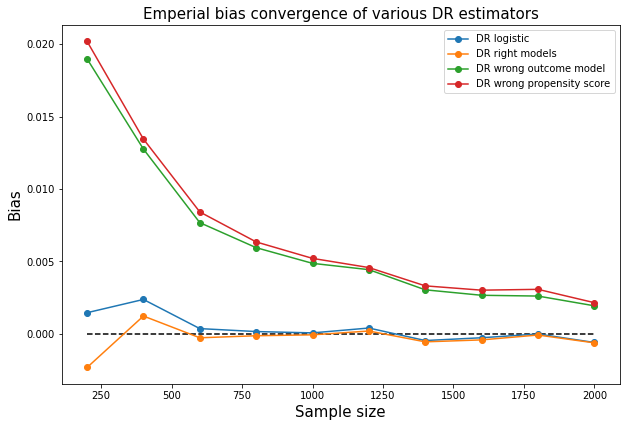
\includegraphics[width = 0.9\columnwidth]{figures/biaspara.png}
    \caption{Simulation results of bias for the various parametric DR estimator specifications}
    \label{figbiaspara}
\end{figure}

\begin{figure}[h!]
    \centering
    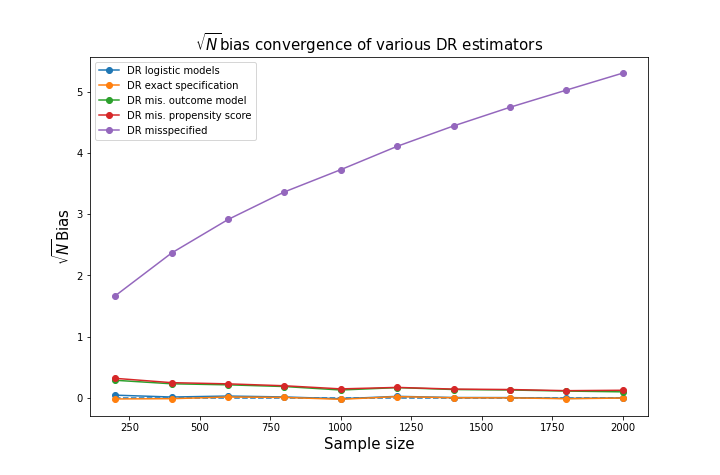
\includegraphics[width = 0.9\columnwidth]{figures/sqrtnpara.png}
    \caption{Simulation results of $\sqrt{N}$bias for the various parametric DR estimator specifications}
    \label{figsqrtnpara}
\end{figure}

Figure \ref{figbiaspara} suggests that the DR estimators with at least one correct specification of the nuisance parameter estimates are indeed consistent as the biases converge to 0 as the sample sizes $N$ get larger -- this is further illustrated in figure \ref{figsqrtnpara}, as we notice that the rates of convergence of the biases are faster than that of $N^{-1/2}$. We also notice that the DR estimation with misspecified propensity score has the poorest convergence out of the 4 estimations, which is in line with the inefficiency that was suggested for such specifications by \citet{kang}. As expected, we also observe poor bias from the DR estimator with both nuisance parameter estimates misspecified, with a diverging $\sqrt{N}$bias curve, confirming that the misspecification of both parameters leads to an inconsistent DR estimator.

\begin{figure}[h!]
    \centering
    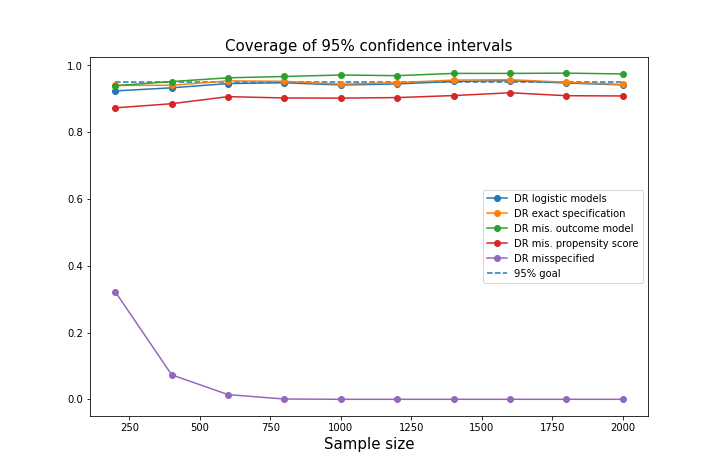
\includegraphics[width = 0.9\columnwidth]{figures/CIpara.png}
    \caption{Simulation results of 95\% CIs coverage for the various parametric DR estimator specifications}
    \label{figCIpara}
\end{figure}

\begin{figure}[h!]
    \centering
    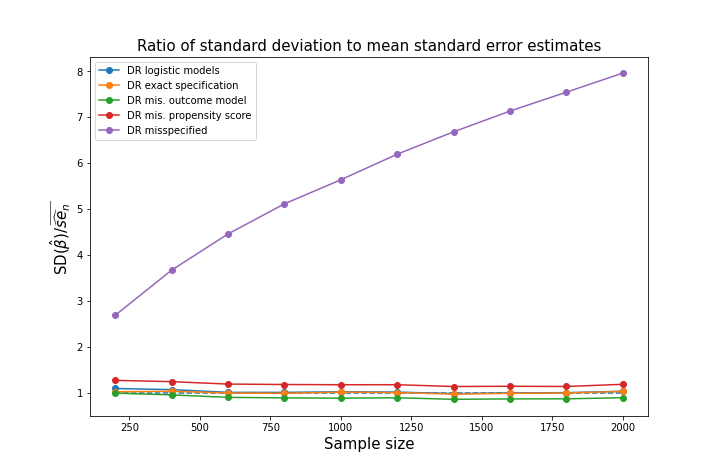
\includegraphics[width = 0.9\columnwidth]{figures/SEpara.png}
    \caption{Accuracy of \citet{lunceford_davidian} SE estimation for the various parametric DR estimator specifications}
    \label{figSEpara}
\end{figure}

Figure \ref{figCIpara} shows the empirical coverage of the 95\% CIs of each estimation, which indeed converges to 95\% for the correctly specified DR estimations. Because the estimation of the SE was specifically for a correctly specified model, the coverage for the DR estimations with one misspecified nuisance parameter model is either too high or too low. To get a better estimation of the SE, one could try other non-model based methods such as bootstrapping, which calculates an estimate of the sample variance based on random samples of the DR estimates. On the flip-side, we notice that for the misspecified DR estimator, as expected the coverage of its CIs converges rapidly to 0, i.e. the CIs based on this misspecified estimator eventually do not contain the true value $\beta$.

Figure \ref{figSEpara} confirms the results we saw above, as we see the ratio of the standard deviation of the DR estimates to the average SE estimator is close to 1 for correctly specified models, hence suggesting a correct calculation of the CI bounds. As for the DR estimations with one misspecified model, this ratio is above or below 1 for \texttt{DR mis. propensity score} and \texttt{DR mis. outcome model} respectively. This indicates that the SE estimation we used is positively or negatively biased, hence giving a CI coverage that is too low for the DR estimator with a misspecified outcome model, or too high for the DR estimator with a misspecified propensity score model. As for the standard deviation to mean SE estimate ratio for the misspecified DR estimator, since the SE estimation is based on correctly specified nuisance parameter estimates, it is to no surprise that it is inconsistent in this case, so the ratio diverges.

\begin{figure}[h!]
    \centering
    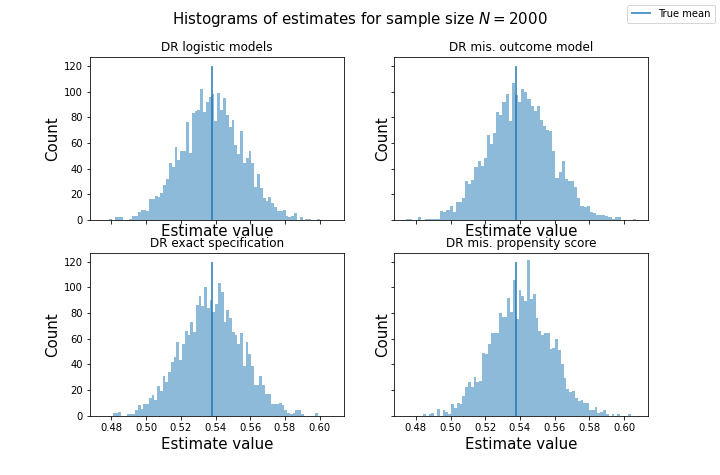
\includegraphics[width = 0.9\columnwidth]{figures/histpara.png}
    \caption{Histograms of parametric DR estimators from simulation results for sample size $N = 2000$}
    \label{fighistpara}
\end{figure}

Figure \ref{fighistpara} suggests that we indeed see asymptotic normality of the distribution, centred at the true mean, of the DR estimators that have at least one correctly specified nuisance parameter model.\\

These results suggest that the parametric approach for setting the nuisance parameter models is a good way of specifying these models, as shown by the low bias and high CI coverage of the estimates. An important advantage of parametric DR estimation is the user-friendly aspect, as we have mentioned previously that logistic or linear regressions models are easy fitting methods to start with, and their theoretical results have been proven in the literature. However we were only able to set the models correctly because we knew the distribution of the data-generative method, and therefore the fact that there was an interactive term between $W_1, W_2$ in the logistic regression model. Had we been given this data set without any information on how it was generated, it would have been time-consuming to find the correct specification of at least one nuisance parameter model. In practice, we would be likely to see results as seen from the DR estimator with both models misspecified, which has no advantage as we saw the CIs eventually didn't contain the true mean. This is where the practicality of ensemble learners from ML tools seem to be a more efficient way of setting these models, which we will cover in the next section.

\clearpage
\section{ML approaches to optimise the DR estimator}

Parametric models for the propensity score and outcome regression are backed by many theoretical results in the literature and are relatively simple models to train thanks to their finite parameter space. However, we have seen in the simulation study above that even a slight misspecification can lead to biased estimations that have CIs almost surely not containing the true mean. Hence the convenience of parametric models is over-weighed by defectiveness under model misspecification \citep{diaz}.

Alternatively, one can use ML models to try to alleviate this bias and CI coverage, as they are often data-adaptive and therefore provide a certain degree of freedom to get a correctly specified model. \citet{ps_SL} have shown that when the propensity score is incorrectly specified, the use of ML tools for specifying the outcome model can still give an unbiased DR estimator, which is an advantage over the parametric scenario, as we had seen that an incorrect propensity score with correct outcome regression was still giving the worse DR estimator in terms of bias in section \ref{para_model}.

Some data-adaptive methods include RFs, Support Vector Machines, kernel regression, outcome weighed learning, Q-learning, neural networks, ensembles of these methods, etc. These methods have been observed to have good empirical performance, but limited theoretical results exist for them. In the following sections, we will take a closer look at the use of RFs and MLPs with various data settings, and see if these data-adaptive methods give better estimates compared to the results from parametric models, even accounting for higher model complexity by adding more covariates to the data.

Note that in nonparametric inference, from \cite{benkeser2017}'s proof of the consistency of the DR estimator, the remainder term 
\begin{align*}
R = R(\hat\pi(\mathbf{W},\hat{\alpha}), \pi(\mathbf{W}), \hat m(\mathbf{W}, \hat\gamma), m(\mathbf{W}))
\end{align*}
of the linearisation of the bias of the DR estimator tends to zero at a rate determined by the rate of convergence of  $\hat\pi(\mathbf{W},\hat{\alpha})$ and  $\hat m(\mathbf{W}, \hat\gamma)$ to $\pi(\mathbf{W})$ and $m(\mathbf{W})$ respectively. Hence the rate of convergence of these nuisance parameter models have a direct effect on the rate of convergence of the DR estimator bias.

\subsection{Using RFs}

RFs are a beginner-friendly ML tool that creates a classification or regression model based on multiple randomly generated decision trees that are combined to make a better prediction than that of a single decision tree. It is easy to use and fit thanks to pre-existing packages in Python and R, and they are also capable of being trained on a data set containing a mix of continuous and categorical features. However, it is not the most time-efficient tool, as the training of the models requires a non-negligible amount of computational power. 

In this section, we will explore the use of RFs for fitting the nuisance parameter models in DR estimation.

\begin{figure}
    \centering
    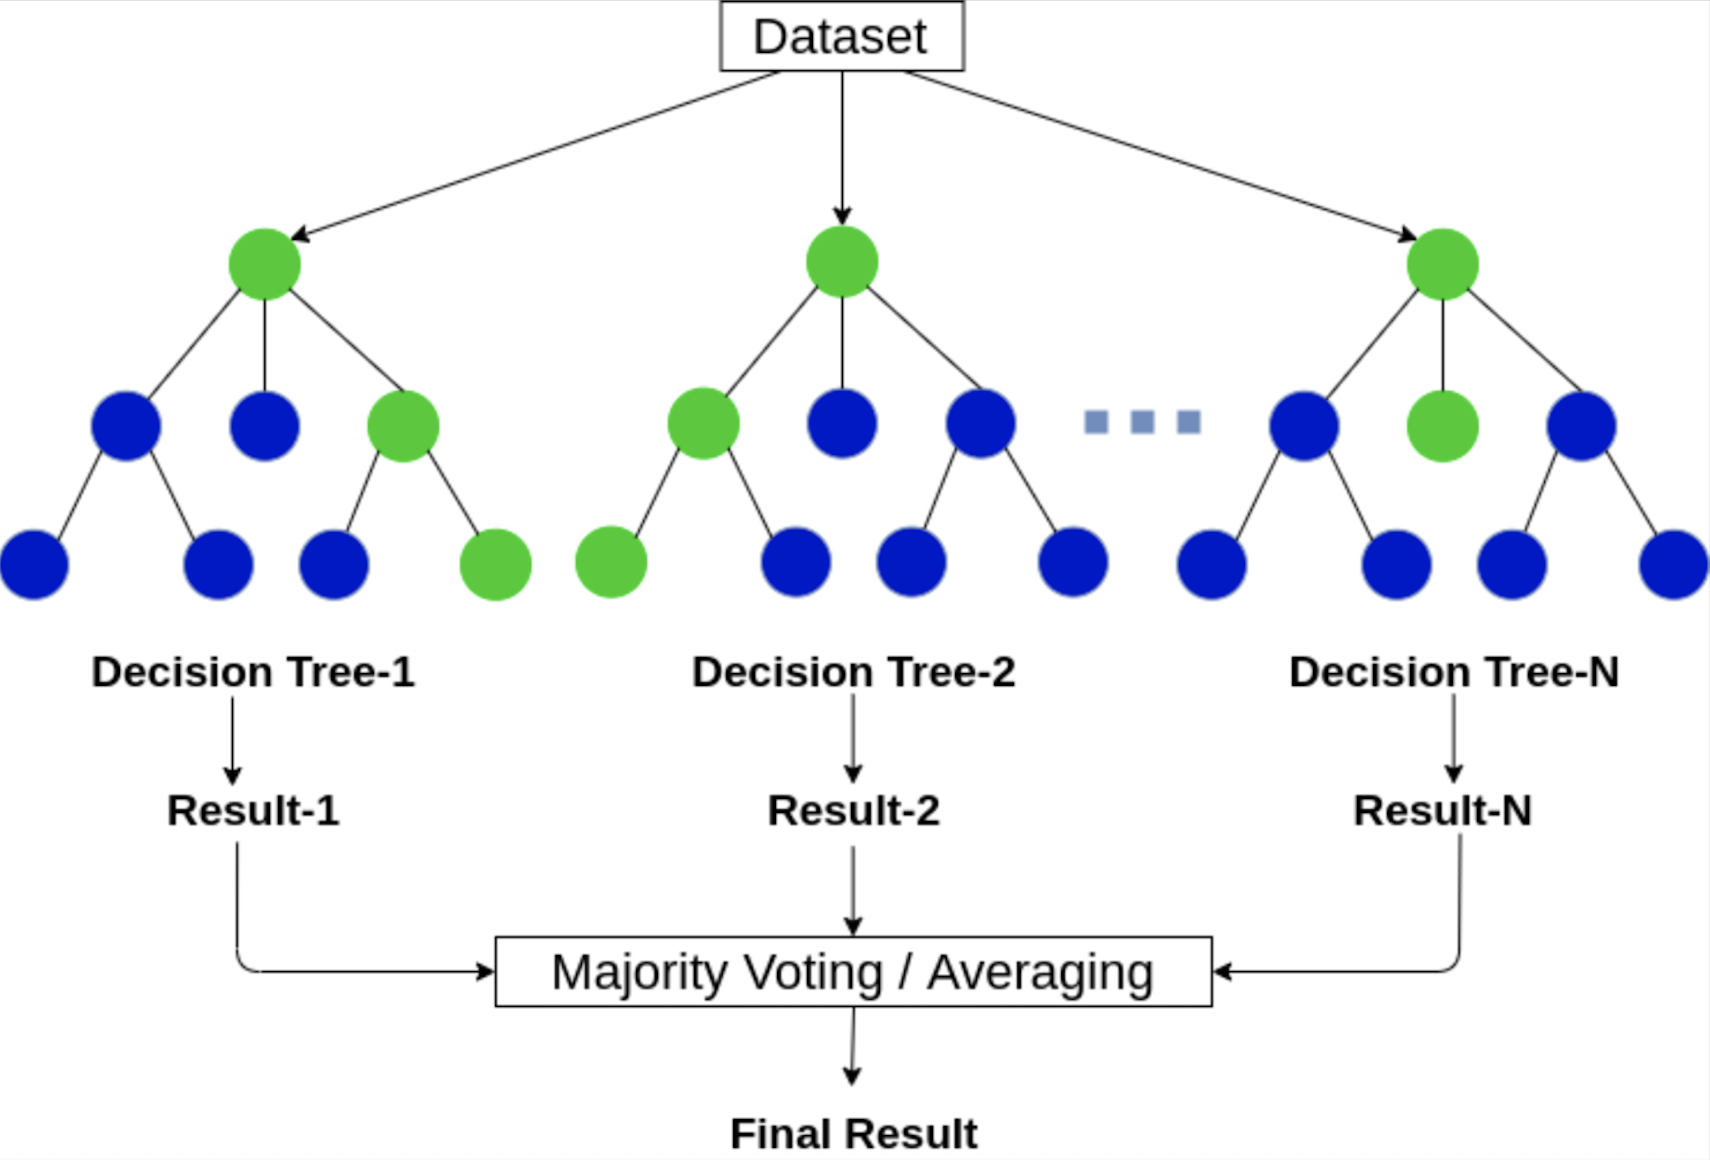
\includegraphics[width = 0.7\columnwidth]{figures/tree.png}
    \caption{Illustration of an RF (source: analyticsvidhya.com)}
    \label{fig:my_label}
\end{figure}



\subsubsection{RF simulation 1: 2 features}

We use the same data generated in section \ref{para_model}, and this time we calculate DR estimators with various nuisance parameter models that are logistic regressions or RFs:
\begin{itemize}
    \item \texttt{DR logistic ps, RF om}: the propensity score model is a correctly specified logistic regression, and the outcome model is an RF. Both models account for the interaction term between $W_1$ and $W_2$ in feature engineering.
    \item \texttt{DR logistic om, RF ps}: the outcome model is a correctly specified logistic regression, and the propensity score is an RF.
    \item \texttt{DR RF}: both the propensity score model and the outcome model are RFs that account for the interaction term between $W_1$ and $W_2$ in feature engineering.
    \item \texttt{DR mis. logistic om, RF ps}: the outcome model is an incorrectly specified logistic regression, and the propensity score model is a correctly specified RF.
    \item \texttt{DR mis. logistic ps, RF om}: the propensity score model is an incorrectly specified logistic regression, and the outcome model is a correctly specified RF.
    \item \texttt{DR mis. RF om, RF ps}: the outcome model is an incorrectly specified RF (i.e no interaction term in feature engineering), and the propensity score model is a correctly specified RF.
    \item \texttt{DR mis. RF ps, RF om}: the propensity score model is an incorrectly specified RF (i.e no interaction term in feature engineering), and the outcome model is a correctly specified RF.
    \item \texttt{DR mis. RF ps \& om}: both the propensity score model and the outcome model are incorrectly specified RFs in feature engineering.
    \item \texttt{DR exact}: both the propensity score model and outcome model are exactly specified by using the distributions from the data generative methods, added for comparison.
\end{itemize}

Each time an RF is specified, it goes through stratified 5-fold cross-validation of RF parameters to input the parameters that give an RF with the best accuracy on the test sets. A summary of the parameters tested by the cross-validation is provided in table \ref{tableRF}. The parameters we cross-validate are the main learning hyperparameters of an RF: the number of decision trees composing the RF, each tree's maximum depth (i.e the maximum number of nodes a decision tree has), and the number of features considered at each branch split in a tree. \\
\begin{table}[]
    \ centering
\begin{tabular}{ |p{3cm}|p{3cm}|p{3cm}| }
 \hline
 \multicolumn{3}{|c|}{RF Cross-validation: Parameter Grid} \\
 \hline
 Number of decision trees & Maximum tree depth (number of splits)  & Maximum    number of features considered at each branch split\\
 \hline
 600, 800, 1000& 10, 15, 20, 25, 30 & 1, 2 \\
 \hline 
\end{tabular}
\caption{Parameter grid of 5-fold cross-validation for RFs in 2-feature simulation}
\label{tableRF}
\end{table}

As before, we obtain an empirical bias by taking the sample mean of 2500 generated estimators of each sample size varying from 200 to 1200 rows in increments of 200. 

\subsubsection*{Results}

\begin{figure}[h!]
    \centering
    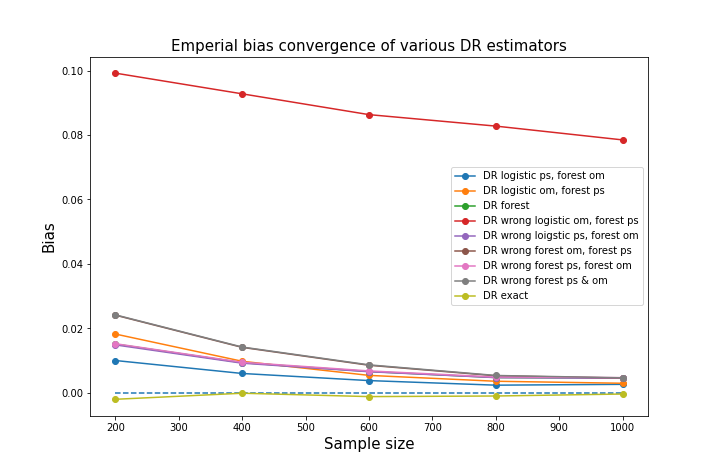
\includegraphics[width = 0.9\columnwidth]{figures/biasRF.png}
    \caption{RF 2-feature simulation results of bias for the various DR estimator specifications}
    \label{figbiasRF}
\end{figure}

\begin{figure} 
    \centering
    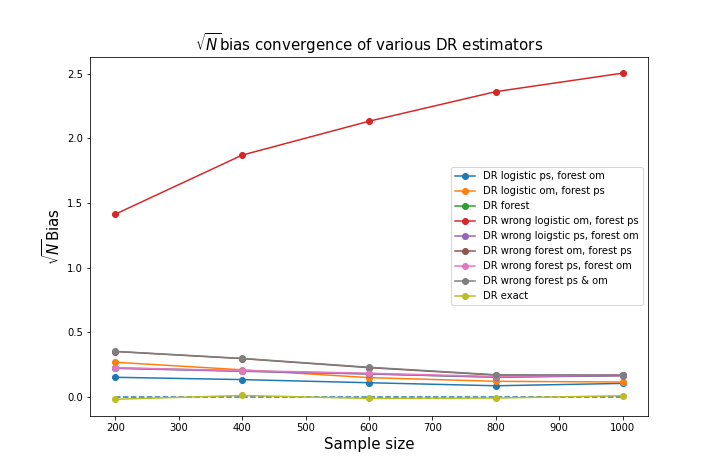
\includegraphics[width = 0.9\columnwidth]{figures/sqrtnRF.png}
    \caption{RF 2-feature simulation results of $\sqrt{N}$bias for the various DR estimator specifications}
    \label{figsqrtnRF}
\end{figure}

We notice in figure \ref{figbiasRF} that the models with RF still provide DR estimates that have bias converging to 0, even when the propensity score model and outcome model are set using an RF that doesn't account for the interaction term. This suggests that the RF can recover the interaction, making it a useful tool in setting the nuisance parameter models. Based on the sample sizes considered, figure \ref{figsqrtnRF} also suggests that these models have biases with a rate of convergence to 0 faster than that of $N^{-1/2}$, which further illustrates the double robustness of the estimators.

We also notice that when the outcome model was an RF and the propensity score model was misspecified with a model that doesn't account for the interaction term, whether that was a logistic regression or an RF, the bias still performs well, which is in line with what \citet{ps_SL} have shown about the recovery of unbiasedness with ML tools for the outcome model when dealing with a misspecified propensity score model. 

However, these figures show an unusual result for the model that had a misspecified logistic outcome model, paired with an RF propensity score model. As we can see in figure \ref{figsqrtnRF}, the bias of this estimate does not converge fast enough, as the plot suggests its rate of convergence to 0 is slower than $N^{-1/2}$, whereas when the misspecification of the outcome model is through an RF, the bias still performs well (its brown line on the graph is overlapped with the grey line). The divergence of the misspecified logistic outcome model from the true outcome model may overpower the convergence of the RF to the true propensity score, so the \cite{benkeser2017} remainder term $R$ has a slow convergence rate, and hence so does the bias of this estimator.

As for the CI coverage results of the various DR estimations in figure \ref{figCIRF}, we notice that their convergence is slower compared to the parametric setting in section \ref{para_model}, and perhaps getting results from larger sample sizes would have shown that they eventually reach the 95\% goal. Figure \ref{figSERF} shows that the standard deviation of the estimated means also converges to the estimated value of the SE at a slower rate than the parametric setting, hence explaining the slowness in CI coverage convergence as well. However for the DR estimator with the misspecified logistic outcome model and RF propensity, this CI coverage simply converges to 0 (with the SE estimate diverging from the standard deviation in \ref{figSERF}), so we eventually do not contain the true value of the sample mean in the CIs based on this specification of the DR estimator. Again, more exploration of DR estimations using a misspecified parametric outcome model and an RF propensity score model is needed to see why this phenomenon is happening.

\begin{figure}[h!]
    \centering
    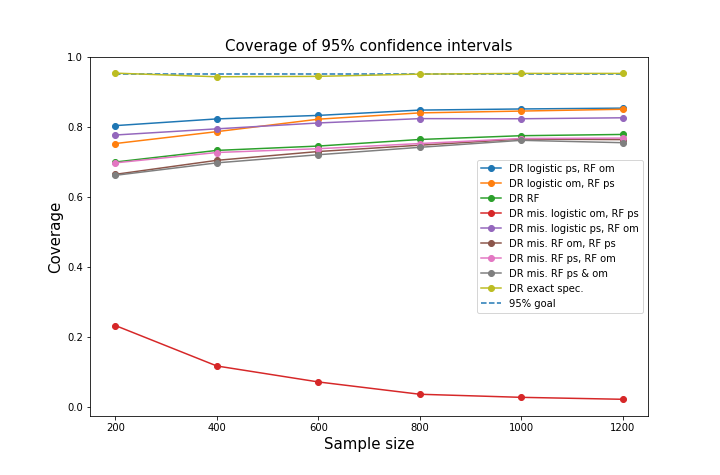
\includegraphics[width = 0.9\columnwidth]{figures/CIRF.png}
    \caption{RF 2-feature simulation results of 95\% CIs coverage for the various DR estimator specifications}
    \label{figCIRF}
\end{figure}

Going back to the DR estimates that were only specified with RFs, figure \ref{fighistRF} suggest asymptotic normality of the distribution of these estimates, like in the parametric setting. \\

Overall the use of RFs in this data set has resulted in consistent DR estimates (except for one estimate mentioned before). Moreover, misspecification of the models by omitting the interaction term was an issue that the RFs easily overcame, as seen in the similar consistency and asymptotic normality results of the RF models that did and did not account for this interaction. This is a non-negligible upgrade from the parametric setting as it suggests that RFs can provide some degrees of freedom for correct model specification. However, the estimates have a high bias compared to the parametric setting. Their CI coverage, and more precisely the \cite{lunceford_davidian} SE estimation could also be improved as we are getting a worse SE estimate to mean sample deviation ratio than in the parametric setting. \cite{benkeser2017} have provided correction procedures to recover almost-nominal CI coverage in inference using nonparametric DR estimation.

\begin{figure}[h!]
    \centering
    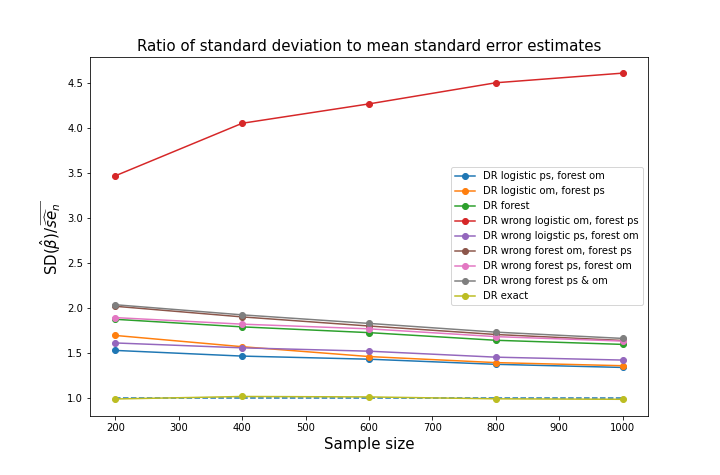
\includegraphics[width = 0.9\columnwidth]{figures/SERF.png}
    \caption{RF 2-feature simulation's accuracy of \citet{lunceford_davidian} SE estimation for the various DR estimator specifications}
    \label{figSERF}
\end{figure}

\begin{figure}[h!]
    \centering
    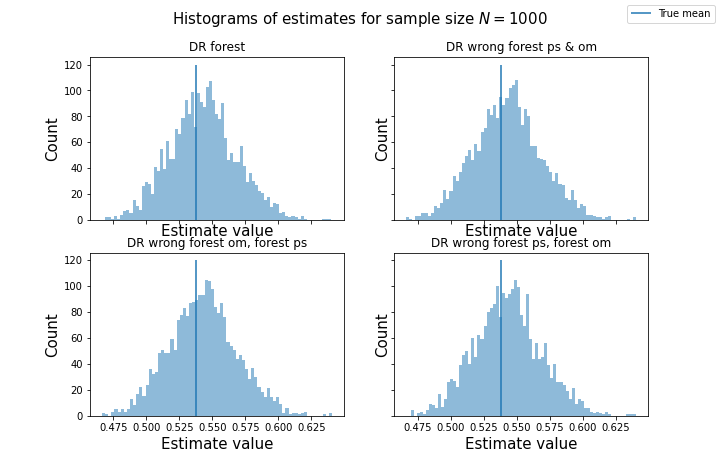
\includegraphics[width = 0.9\columnwidth]{figures/histRF.png}
    \caption{RF 2-feature simulation's histograms of DR estimates for sample size $N = 1200$}
    \label{fighistRF}
\end{figure}

\clearpage
\subsubsection{RF simulation 2: 4 features} \label{RF simu 2}

This time we increase the complexity of our DR estimation by adding two new features to the data-generative method from the previous section. We now have $\mathbf{W} = (W_1,W_2,W_3,W_4)$ where $W_1,W_2$ are as before, $W_3$ follows a standard normal distribution and $W_4$ follows an exponential distribution with mean 1. The features are mutually independent. The new true propensity score model is 
\begin{align*}
    \pi(\mathbf{W}) = P(R = 1 |\mathbf{W} = (w_1,w_2, w_3,w_4)) = \expit(-w_1 + 2w_1w_2 - w_3 + 2w_3w_4)
\end{align*}
and the new true outcome model is 
\begin{align*}
    m(\mathbf{W}) &= E(Y|\mathbf{W}, R=1) \\
    & = \expit(0.2 - w_1 + 2w_1w_2 - w_3 + 2w_3w_4)
\end{align*}

Note that the true outcome mean $\beta$ remains approximately the same at 0.53 despite the added features.

We ran simulations using the same combination of nuisance parameter model settings as in the 2-feature simulation, but this time when we refer to misspecified specification, it means the model didn't account for both interaction terms $W_1W_2$ and $W_3W_4$. The cross-validation for the RFs was also expanded to consider up to 4 features at a time in each split. 

\subsubsection*{Results}

Unlike the simulation with 2 features, this time with the addition of 2 new features we obtained estimates that had poor convergence rates. Figure \ref{figbiasRF_moreW} already suggests higher bias in the estimators and deceleration of the bias rate of convergence compared to the simulation with 2 features. This is further illustrated in figure \ref{figsqrtnRF_moreW} as the divergence of the bias elevated to $N^{1/2}$ suggest that the rate of convergence to 0 is slower than $N^{-1/2}$. The only estimator that performed well in this setting, based on the sample sizes considered, is the estimator with a correct logistic outcome model and an RF propensity score model that accounts for the interactions terms (orange line in the plots). 

\begin{figure}[h!]
    \centering
    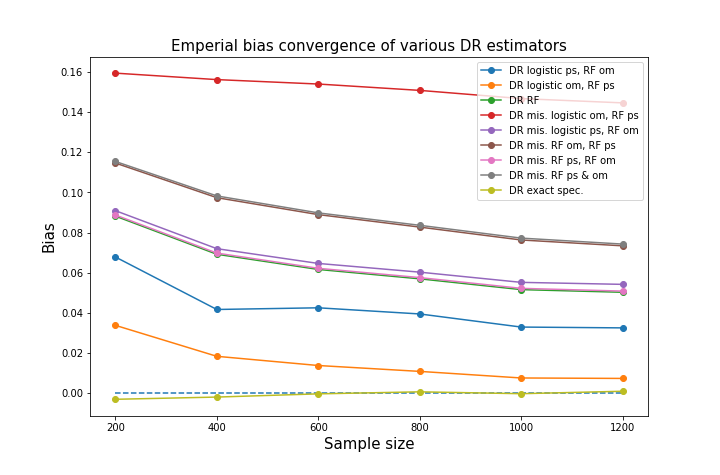
\includegraphics[width = 0.9\columnwidth]{figures/biasRF_moreW.png}
    \caption{RF 4-feature simulation results of bias for the various DR estimator specifications}
    \label{figbiasRF_moreW}
\end{figure}

\begin{figure}[h!]
    \centering
    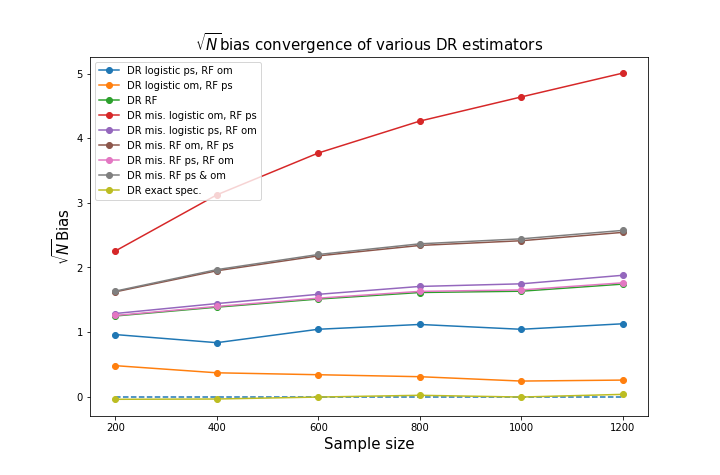
\includegraphics[width = 0.9\columnwidth]{figures/sqrtnRF_moreW.png}
    \caption{RF 4-feature simulation results of $\sqrt{N}$bias for the various DR estimator specifications}
    \label{figsqrtnRF_moreW}
\end{figure}

Unsurprisingly, the convergence to 95\% CI coverage is also poor as seen in figure \ref{figCIRF_moreW}, and many of the estimators have a CI coverage converging to 0. This is further illustrated by the divergence of the SE estimate from the true deviation as seen in figure \ref{figSERF_moreW}. Even for the estimator that had a fast enough bias convergence (orange in plots), the convergence to a 95\% coverage of its CIs is relatively slow, and from sample size 1000 to 1200, there is a slight decrease in coverage. This might suggest a worsening of the CI coverage in larger samples.

\begin{figure}[h!]
    \centering
    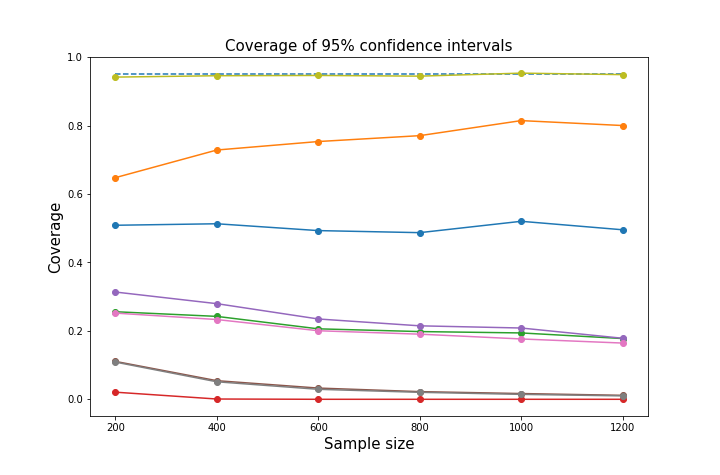
\includegraphics[width = 0.9\columnwidth]{figures/CIRF_moreW.png}
    \caption{RF 4-feature simulation results of 95\% CIs coverage for the various DR estimator specifications}
    \label{figCIRF_moreW}
\end{figure}

\begin{figure}[h!]
    \centering
    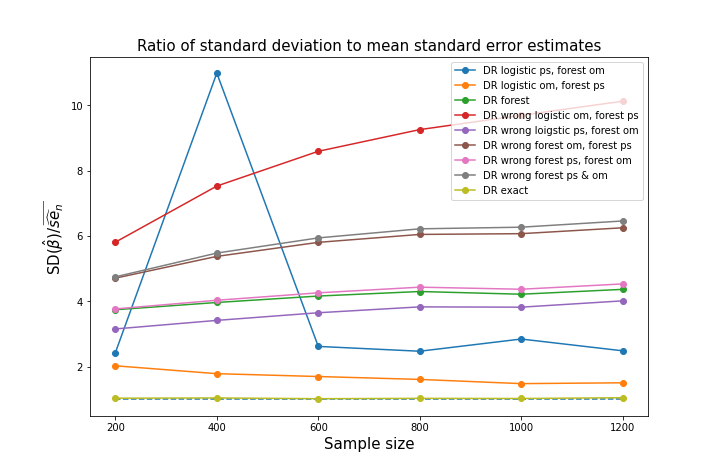
\includegraphics[width = 0.9\columnwidth]{figures/SERF_moreW.png}
    \caption{RF 4-feature simulation's accuracy of \citet{lunceford_davidian} SE estimation for the various DR estimator specifications}
    \label{figSERF_moreW}
\end{figure}

It is with no surprise that due to the slowness of the convergences, a normal distribution centred at the true mean hasn't been achieved for the largest sample size considered in the simulation, in particular for the DR estimators involving RFs only, as seen in figure \ref{fighistRF_moreW}. \\

\begin{figure}[h!]
    \centering
    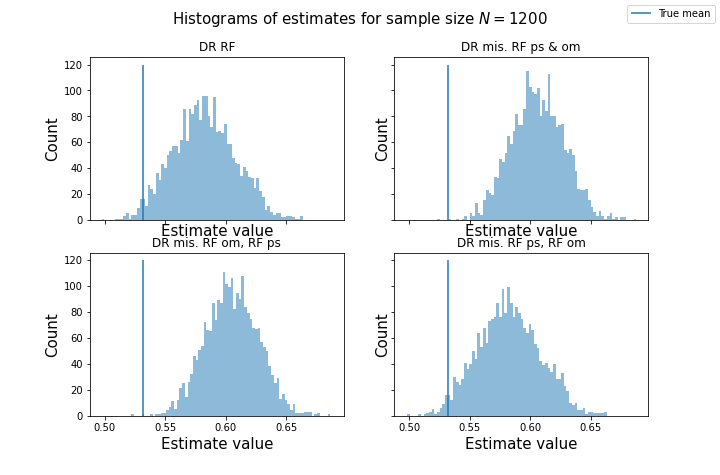
\includegraphics[width = 0.9\columnwidth]{figures/histRF_moreW.png}
    \caption{RF 4-feature simulation's histograms of DR estimates for sample size $N = 1200$}
    \label{fighistRF_moreW}
\end{figure}

Overall, doubling the number of features has resulted in poor bias and slow convergence of the DR estimates to the true value of the mean. This may be an example of the so-called curse of dimensionality \citep{Wasserman2006}: by doubling the number of features, the complexity of training the RFs overcomes correct classification or regression, leading to the poor convergence of our DR estimates to the true value. Had the added features $W_3, W_4$ had a smaller range of values, we might have alleviated the complexity of the classification problem. Although we had found good results using RFs in the 2-features case, one must take into account the complexity of the dataset and classification/regression problem before choosing to use an RF to set the nuisance parameter models of a DR estimator.

\clearpage
\subsection{Using MLPs}
\begin{figure}[h!]
    \centering
    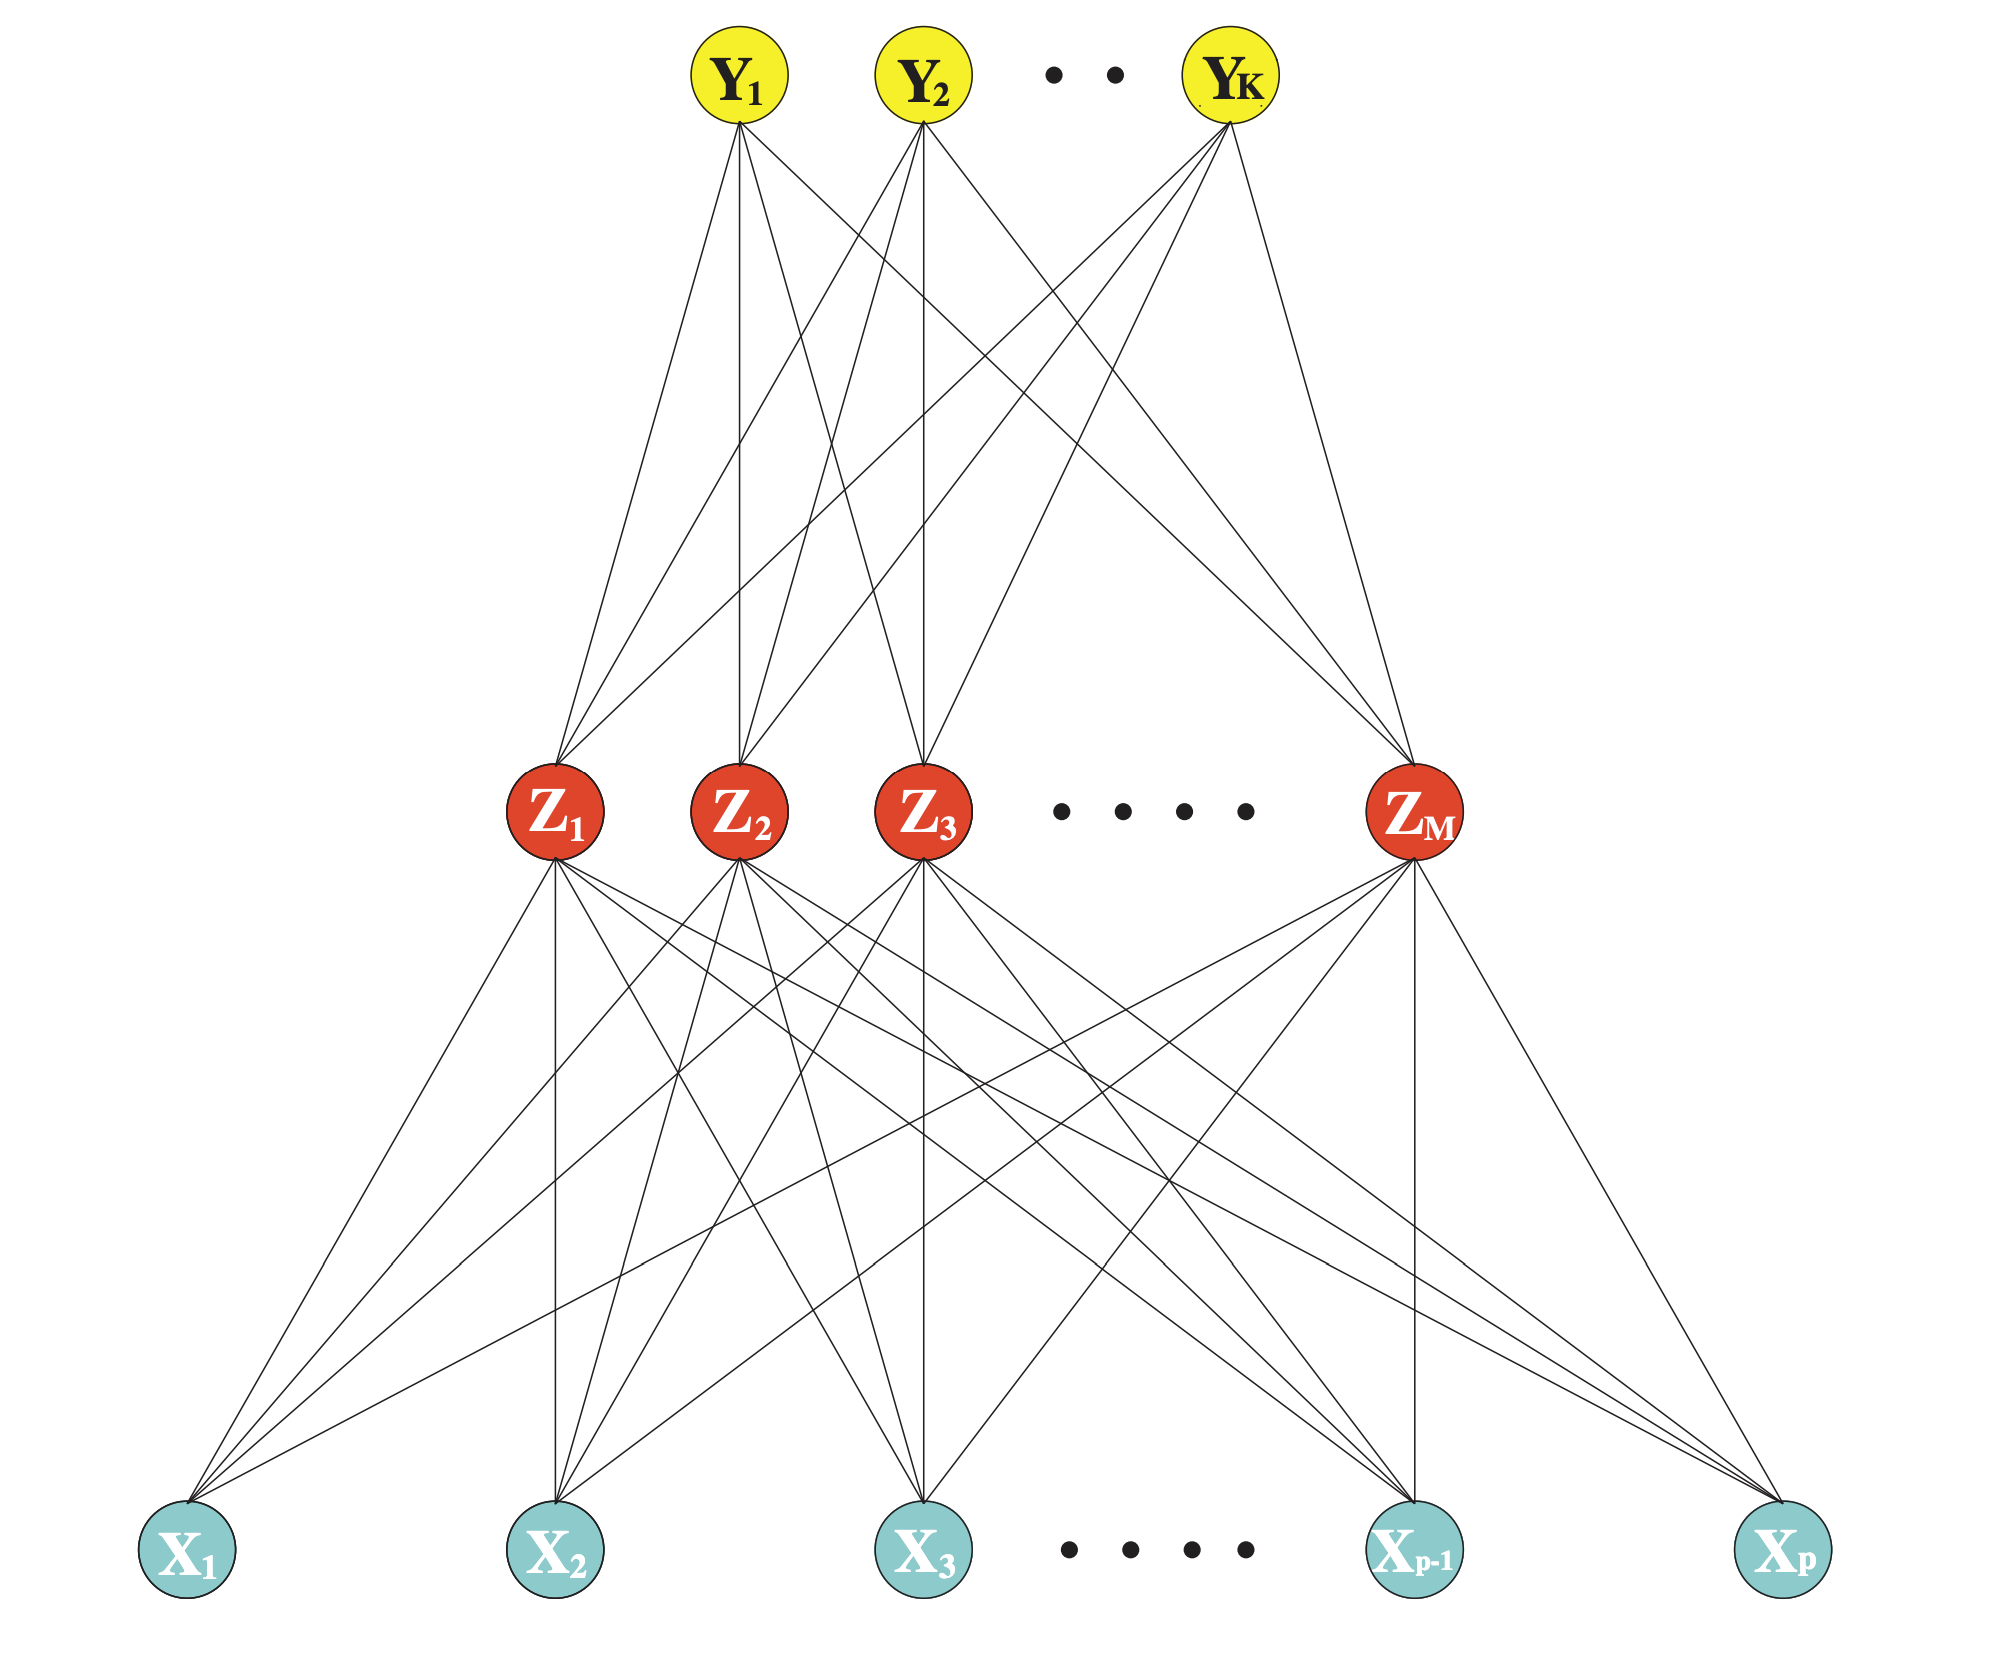
\includegraphics[width = 0.7\columnwidth]{figures/Screenshot 2021-05-26 at 19.21.43.png}
    \caption{Network diagram of a single layer perceptron \citep{hastieESL}}
    \label{fignn}
\end{figure}

This section is motivated by the publication by \citet{setoguchi-nn} suggesting that neural networks reduce the bias of propensity score models compared to logistic regression, and hence should also alleviate the bias of the DR estimator. This time we are using MLPs, a type of forward-feeding artificial neural network. As mentioned by \citet{hastieESL}, there is a lot of popularity surrounding neural networks lately, and like RFs, they are easy to implement in Python thanks to the scikit-learn module. The training time of an MLP is also faster than that of an RF for models with a small number of features. 

In a classification problem, there are $K$ output nodes at the end of the network diagram corresponding to the $K$ categories the output $Y$ can be in. The first layer of nodes in the diagram corresponds to the $p$ input features. Then, each node in the hidden layers of the network is created as a linear combination of the previous layer's nodes. At the end of the network, the output nodes are created as functions of linear combinations of the last hidden layer's nodes. An illustration of the network diagram of a single layer perceptron is provided in figure \ref{fignn}, taken from \textit{The Elements of Statistical Learning} by \citet{hastieESL}.

In the following sections, we will evaluate the use of MLPs for DR estimation, through simulations on the data sets we have encountered in the previous sections.

\subsubsection{MLP simulation 1: 2 features} \label{MLP simu 1}

We go back to the data structure that had 2 features $W_1, W_2$, and we wish to see what happens to the consistency of the DR estimates when we use MLPs for the propensity score model or outcome model. The various DR estimates based on MLP nuisance parameter models are as follows: 
\begin{itemize}
    \item \texttt{DR logistic ps, MLP om}: the propensity score model is a correctly specified logistic regression, and the outcome model is an MLP. Both model account for the interaction term between $W_1$ and $W_2$
    \item \texttt{DR logistic om, MLP ps}: the outcome model is a correctly specified logistic regression, and the propensity score model is an MLP.
    \item \texttt{DR MLP}: both the propensity score model and the outcome model are MLPs that account for the interaction term between $W_1$ and $W_2$.
    \item \texttt{DR mis. logistic om, MLP ps}: the outcome model is an incorrectly specified logistic regression, and the propensity score model is a correctly specified MLP.
    \item \texttt{DR mis. logistic ps, MLP om}: the propensity score model is an incorrectly specified logistic regression, and the outcome model is a correctly specified MLP.
    \item \texttt{DR mis. MLP om, MLP ps}: the outcome model is an incorrectly specified MLP (i.e no interaction term), and the propensity score model is a correctly specified MLP.
    \item \texttt{DR mis. MLP ps, MLP om}: the propensity score model is an incorrectly specified MLP (i.e no interaction term), and the outcome model is a correctly specified MLP.
    \item \texttt{DR mis. MLP ps \& om}: both the propensity score model and the outcome model are incorrectly specified MLPs.
    \item \texttt{DR exact}: both the propensity score model and outcome model are exactly specified by using the distributions from the data generative methods, added for comparison.
\end{itemize}

Like with RFs, the MLPs also go through a 5-fold cross-validation process to tune model parameters. A summary of the range of parameters tested by the cross-validation is provided in table \ref{tableMLP}. The learning rate parameter determines the rate of node weight updates at hidden layers, 'activation' determines the activation function of each hidden layer and 'alpha' is the penalty parameter of the MLP.

\begin{table}[h!]
    \centering
\begin{tabular}{ |p{3cm}|p{3cm}|p{3cm}|p{3cm}| }
 \hline
 \multicolumn{4}{|c|}{MLP Cross-validation: Parameter Grid} \\
 \hline
 Hidden layer sizes & Learning rate & Activation & Alpha\\
 \hline
 3 layers of size (10, 20, 30), 2 layers of size (50, 50), 1 layer of size 100 & Constant, invscaling, adaptive & Logistic, relu, tanh & $10^{-1}$, $10^{-2}$, $10^{-3}$, $10^{-4}$ \\
 \hline 
\end{tabular}
\caption{Parameter grid of 5-fold cross-validation for MLPs in 2-feature simulation}
\label{tableMLP}
\end{table}

\subsubsection*{Results}

\begin{figure}[h!]
    \centering
    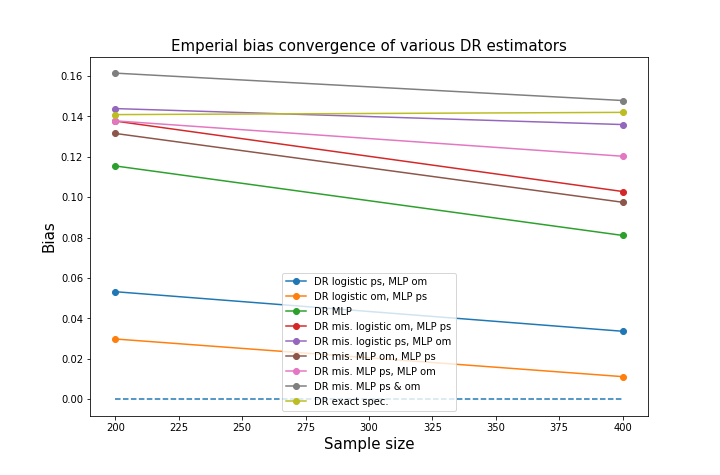
\includegraphics[width = 0.9\columnwidth]{figures/biasMLP.png}
    \caption{MLP 2-feature simulation results of bias for the various DR estimator specifications}
    \label{figbiasMLP}
\end{figure}

\begin{figure}[h!]
    \centering
    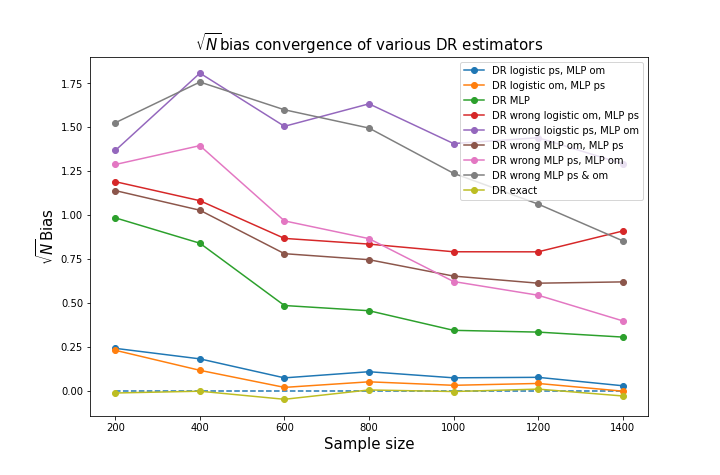
\includegraphics[width = 0.9\columnwidth]{figures/sqrtnMLP.png}
    \caption{MLP 2-feature simulation results of $\sqrt{N}$bias for the various DR estimator specifications}
    \label{figsqrtnMLP}
\end{figure}

In figure \ref{figbiasMLP} we notice that most estimates involving at least one MLP nuisance parameter models have a bias seeming to converge towards zero. Excluding the DR estimate with exact specification, the estimate with the lowest bias is the one that had a logistic outcome regression and an MLP propensity score model, and it outperforms the estimate with the logistic propensity score model. This goes in line with the findings of \citet{setoguchi-nn} about an MLP propensity score model having lower bias than with logistic regression. The DR estimate set with correct MLPs for both nuisance parameter models performs well in terms of bias as well, although the convergence to 0 bias plateaus as sample sizes get larger. The DR estimate with misspecified logistic outcome model and MLP propensity score model (red plotline) has a U-shaped bias curve, suggesting a worsening bias in larger samples. Looking at figure \ref{figsqrtnMLP}, the bias convergence to 0 for these estimates seem to be faster than that of $N^{-1/2}$ for most estimates as shown by the downward trend of the $\sqrt{N}$bias curves, while the estimate with misspecified logistic outcome model and MLP propensity score model shows sign of diverging, in line with what we saw in figure \ref{figbiasMLP}. The DR estimator with misspecified logistic propensity score model and MLP outcome model, \texttt{DR mis. logistic ps, MLP om} (purple line on the plots) has one of the highest bias among these estimators, but the convergence of the bias at a higher speed than $N^{-1/2}$ suggests that the incorrect specification was overcome by the MLPs and so the estimate is still consistent, even though it will converge towards the true mean at a slower pace than the estimates with at least one correct MLP specification. Another notable estimate is the one with a misspecified MLP propensity score model and MLP outcome model (pink line in plots). Even though this estimate starts at high bias, the latter is seeming to quickly converge to 0.

\begin{figure}[h!]
    \centering
    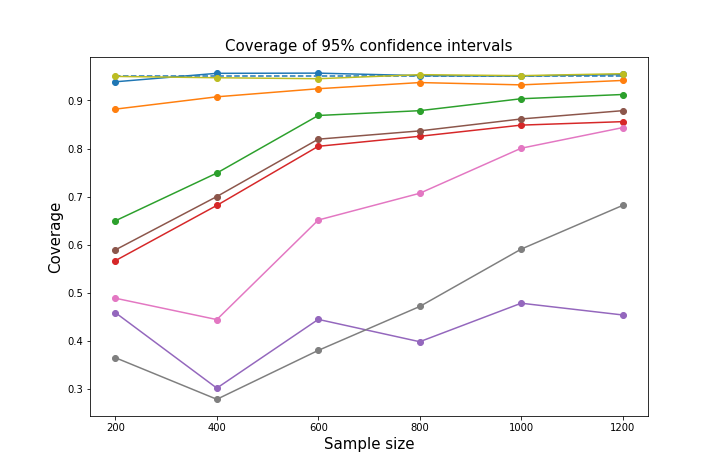
\includegraphics[width = 0.9\columnwidth]{figures/CIMLP.png}
    \caption{MLP 2-feature simulation results of 95\% CIs coverage for the various DR estimator specifications}
    \label{figCIMLP}
\end{figure}

The CI coverage plot in figure \ref{figCIMLP} also shows interesting results. \texttt{DR logistic om, MLP ps}, \texttt{DR logistic ps, MLP om}, \texttt{DR mis. MLP om, MLP ps} and \texttt{DR mis. MLP ps \& om} (in blue, orange pink and grey) have CI coverage tending to the 95\% goal, with the estimates with higher bias generally tending to 95\% coverage at a slower rate. Their SE estimates, as seen \ref{figSEMLP}, also suggest being tending towards the true value. On the other hand, we see an upside-down U-shape from the CI coverage and SE estimate curves of \texttt{DR MLP, DR logistic om, MLP ps, DR mis. MLP om, MLP ps} (in green, red and brown), suggesting a worsening CI coverage for larger sample sizes. These plots seem to suggest that a misspecification of the MLP for the propensity score model is providing a better CI coverage convergence of the DR estimates. The DR estimate struggling to get up to high CI coverage the most here is again \texttt{DR mis. logistic ps, MLP om}. We see from figure \ref{figSEMLP} that non-surprisingly, its SE estimate is converging to the true standard deviation at a slow pace as well, given the considered sample sizes. 

\begin{figure}[h!]
    \centering
    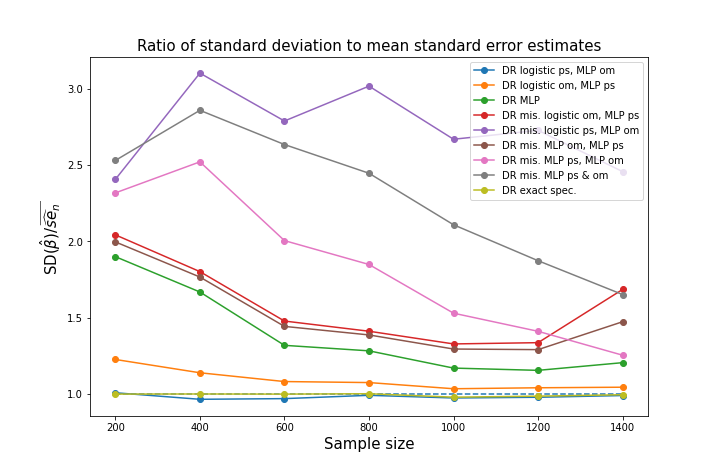
\includegraphics[width = 0.9\columnwidth]{figures/SEMLP.png}
    \caption{MLP 2-feature simulation's accuracy of \citet{lunceford_davidian} SE estimation for the various DR estimator specifications}
    \label{figSEMLP}
\end{figure}

Taking a particular look at the histograms of the DR estimates involving only MLPs for the largest sample size considered, we notice that although \texttt{DR MLP} and \texttt{DR mis. MLP om, MLP ps} have distributions almost centred at the true mean, we know from the diverging trend of their CI coverage at larger samples that these histograms will be less and less centred at the true mean as we increase sample size, so we wouldn't expect asymptotic normality from these. On the other hand, from the way the bias and CI coverage of \texttt{DR mis. MLP ps \& om} and \texttt{DR mis. MLP ps, MLP om} were converging, we are likely to get an asymptotic normal distribution from these estimates, although at a slower rate than the parametric setting. Since \texttt{DR mis. MLP ps \& om} had higher bias, its histogram in figure \ref{fighistMLP} is less centered at the true value than that of \texttt{DR mis. MLP ps, MLP om} at the given sample size. The more centred estimator likely has one or both nuisance parameter models converging faster to the true nuisance parameters than that of the less centred estimator's, making the remainder term in \cite{benkeser2017}'s bias linearisation converge faster to 0.

\begin{figure}[h!]
    \centering
    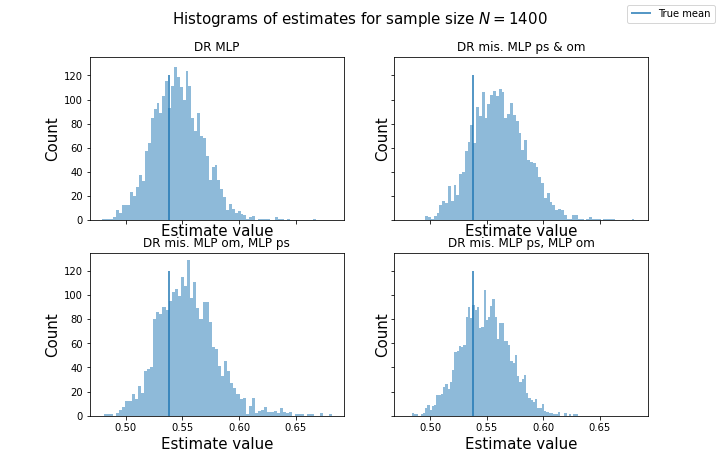
\includegraphics[width = 0.9\columnwidth]{figures/histMLP.png}
    \caption{MLP 2-feature simulation's histograms of DR estimates for sample size $N = 1400$}
    \label{fighistMLP}
\end{figure}

\clearpage
\subsubsection{MLP simulation 2: 4 features}

Like in the second RF simulation from section \ref{RF simu 2}, we now wish to illustrate the efficacy of MLPs in the DR estimations from section \ref{MLP simu 1}, with two features $W_3, W_4$ added to the previous simulation's data. The distributions of $W_1,..., W_4$ haven't changed from section \ref{RF simu 2}. We also maintain the same cross-validation grid from the first MLP simulation in section \ref{MLP simu 1}. As in section \ref{RF simu 2}, when we refer to a misspecified nuisance parameter model, we mean that both the interactions between $W_1, W_2$ and $W_3, W_4$ are not accounted for in the feature engineering of the model.

\textit{The author apologises for the lack of data points at sample sizes $N = 800, 1200$, as they ran into computational issues for these particular sample sizes that could not be fixed in time.}

\subsubsection*{Results}

\begin{figure}[h!]
    \centering
    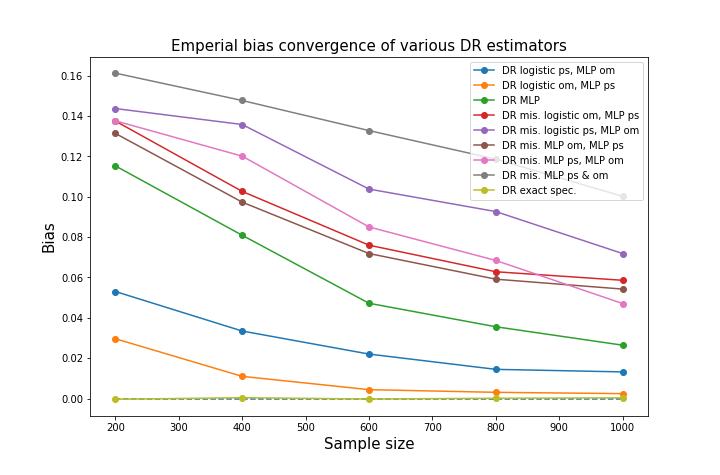
\includegraphics[width = 0.9\columnwidth]{figures/biasMLP_moreW.png}
    \caption{MLP 4-feature simulation results of bias for the various DR estimator specifications}
    \label{figbiasMLP_moreW}
\end{figure}

\begin{figure}[h!]
    \centering
    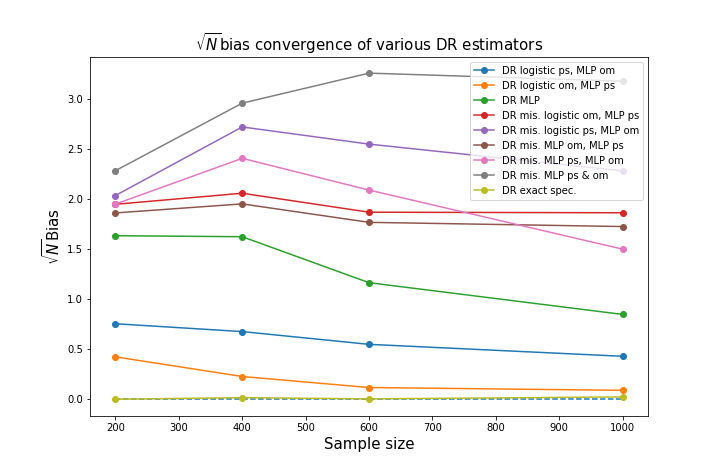
\includegraphics[width = 0.9\columnwidth]{figures/sqrtnMLP_moreW.png}
    \caption{MLP 4-feature simulation results of $\sqrt{N}$bias for the various DR estimator specifications}
    \label{figsqrtnMLP_moreW}
\end{figure}

With the added complexity from having 4 features, the DR estimates involving MLPs are still showing downward trends in their bias as seen in figure \ref{figbiasMLP_moreW}, although the biases are higher and tend to 0 at a slower rate than the 2-feature case from the previous simulation. Note in figure \ref{figsqrtnMLP_moreW} that the DR estimates have downward-trending $\sqrt{N}$bias curves, suggesting that the rate of convergence of their bias is at least as fast as that of $N^{-1/2}$. The only exception is the DR estimate that had misspecified MLPs for both nuisance parameter models (in grey on the plot), for which we have an upward $\sqrt{N}$bias trend, which suggests that its bias has a convergence rate slower than that of $N^{-1/2}$.

\begin{figure}[h!]
    \centering
    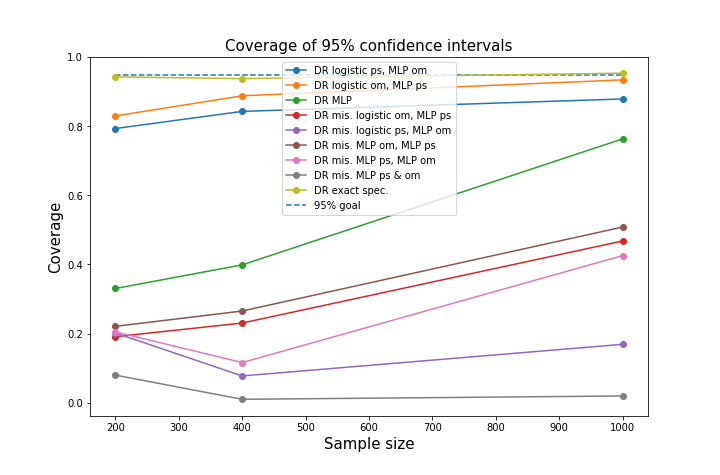
\includegraphics[width = 0.9\columnwidth]{figures/CIMLP_moreW.png}
    \caption{MLP 4-feature simulation results of 95\% CIs coverage for the various DR estimator specifications}
    \label{figCIMLP_moreW}
\end{figure}

\begin{figure}[h!]
    \centering
    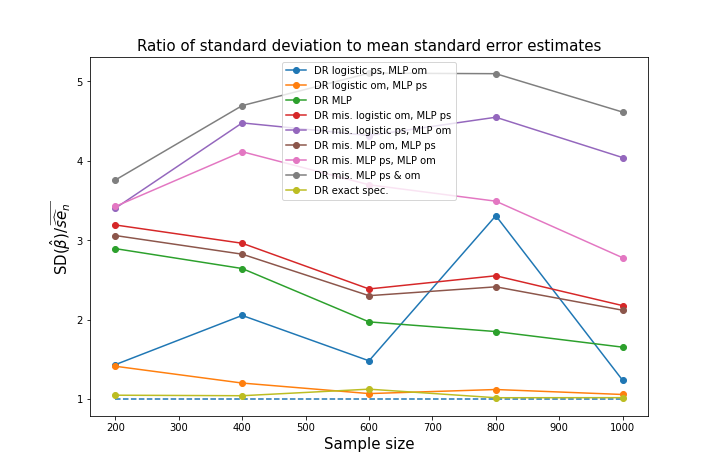
\includegraphics[width = 0.9\columnwidth]{figures/SEMLP_moreW.png}
    \caption{MLP 4-feature simulation's accuracy of \citet{lunceford_davidian} SE estimation for the various DR estimator specifications}
    \label{figSEMLP_moreW}
\end{figure}

As for CI coverage performance, figure \ref{figCIMLP_moreW} suggests that the DR estimator with both MLP nuisance parameter models that account for the feature interaction (in green on the plot) has low CI coverage, but this coverage is converging to the nominal 95\% value at a relatively fast rate. The ratio of its mean SE estimate to the sample standard deviation is also tending towards 1, as seen in figure \ref{figSEMLP_moreW}. The DR estimates with exact or correct logistic models are reaching high coverage as expected because at least one of the models is correctly specified. For the rest of the estimators involving MLPs (in brown, pink, red, purple), their CI coverage is substantially lower, but again we see an upward trend of this coverage, although at a slower rate. Their SE estimate to standard deviation ratio tending to 1 at a slow rate, as seen in figure \ref{figSEMLP_moreW}, go in line with this slow upward trend in their CI coverage. Unsurprisingly, the DR estimate with misspecified MLP nuisance parameter models has very poor CI coverage as its SE estimate to standard deviation ratio is not converging to 1. Unlike in the 2-feature case, this time misspecification of the interaction terms in both MLP nuisance parameter models resulted in poor CI coverage. This is likely because not accounting for 2 interaction terms in the model specification in the 4-feature case was more penalising to the MLPs' ability to recover them, than not accounting for just 1 in the 2-feature case.

\begin{figure}[h!]
    \centering
    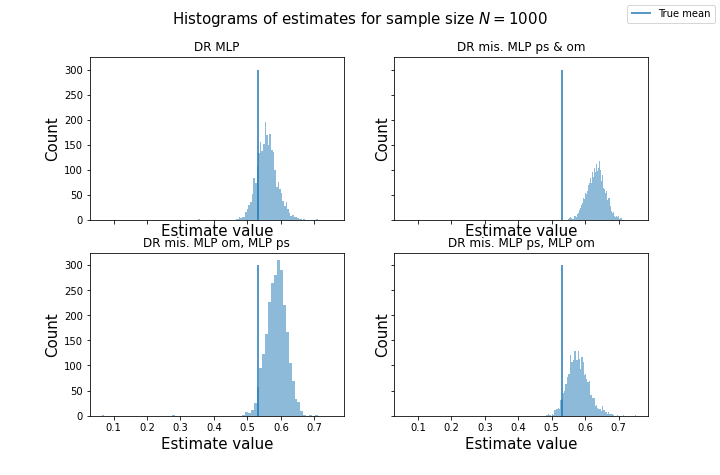
\includegraphics[width = 0.9\columnwidth]{figures/histMLP_moreW.png}
    \caption{MLP 4-feature simulation's histograms of DR estimates for sample size $N = 1200$}
    \label{fighistMLP_moreW}
\end{figure}

Due to its lower bias, \texttt{DR MLP} has the most centred histogram at a high sample size compared to the other 3 DR estimates involving only MLPs, as seen in figure \ref{fighistMLP_moreW}. \texttt{DR mis. MLP ps \& om}, having the highest bias, has a histogram of values that is heavily skewed to the right. It is also the case for the DR estimates with one misspecified MLP, but we expect these to become more centred at the true mean as we increase the sample size.

Overall, the complexity from having doubled the number of features relatively did not penalise MLPs too much in terms of their convergence to the true nuisance parameters, which has led to DR estimates that, although having higher bias and lower CI coverage, still show signs of converging to the true mean at a slower rate than the 2 feature case.
\clearpage
\subsection{Discussion}

\subsubsection{2-feature case} \label{2 features}

\begin{figure}[h!]
    \centering
    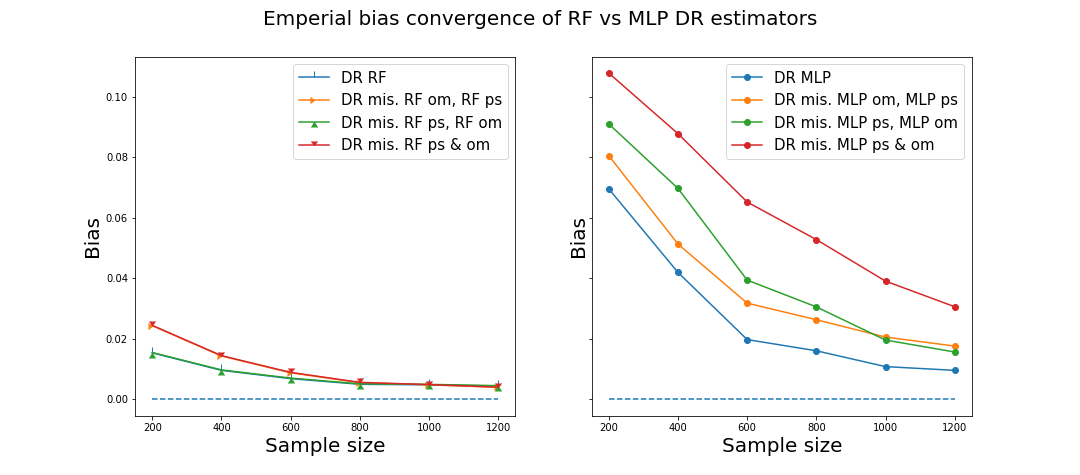
\includegraphics[width = 0.9\columnwidth]{figures/biascompare.png}
    \caption{Comparing bias performance on simulations with 2 features}
    \label{biascompare}
\end{figure}

\begin{figure}[h!]
    \centering
    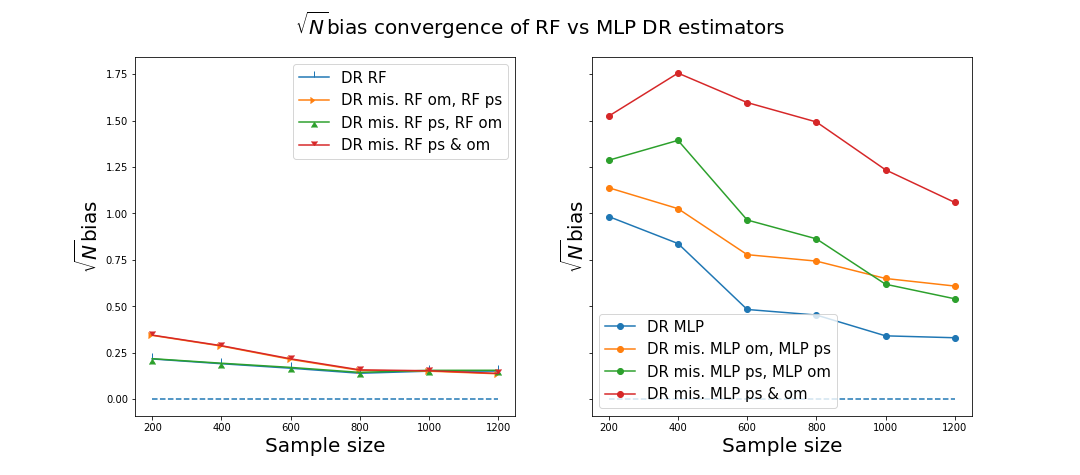
\includegraphics[width = 0.9\columnwidth]{figures/sqrtncompare.png}
    \caption{Comparing $\sqrt{N}$bias performance on simulations with 2 features}
    \label{sqrtncompare}
\end{figure}

Figure \ref{biascompare} and \ref{sqrtncompare} suggests that in the 2-feature case, DR estimates involving RFs had lower bias than the DR estimates involving MLPs, but these biases converge to 0 at a slower rate than the biases of the MLP-based DR estimates. Note that with both ML tools, not accounting for the interaction term $W_1W_2$ in both nuisance parameter models has resulted in higher bias in the DR estimation, compared to when at least one of the nuisance parameter ML models accounted for the interaction term. If the user has no information on the distribution of the outcome and the propensity score and is uncertain of whether an interaction exists, they could account for this interaction term in one of the two ML nuisance parameter models to ensure at least one of the ML models is correctly specified. In the parametric approach, the user needed to get both the parametric distribution assumption and the interaction term correctly specified; in the nonparametric approach with RFs and MLPs, the user only needs to get the interaction term correctly specified, hence reducing the chance of misspecification compared to the parametric method.

\begin{figure}[h!]
    \centering
    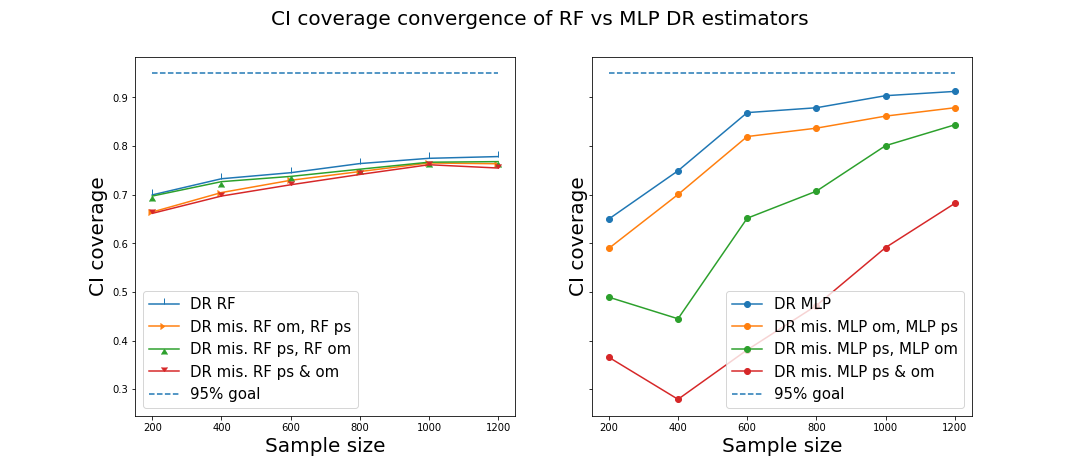
\includegraphics[width = 0.9\columnwidth]{figures/CIcompare.png}
    \caption{Comparing CI coverage performance for RFs vs MLPs on simulation with 2 features}
    \label{CIcompare}
\end{figure}
 
As for CIs constructed from these estimators, the DR estimators with RFs start at a higher CI coverage value but fail to converge fast enough to the 95\% coverage goal value as seen in figure \ref{CIcompare}. However, the DR estimators with MLPs start at low CI coverage but converge to the nominal value at a faster rate.

To summarise, when choosing between RFs and MLPs for nuisance parameter model setting for this specific data set, if one seeks to have DR estimations with lower bias, one should prioritise RFs; if one wishes to construct CIs with high coverage, especially with large sample sizes, one should turn towards using MLPs in their DR estimation.

\subsubsection{4-feature case} \label{4 features}

\begin{figure}[h!]
    \centering
    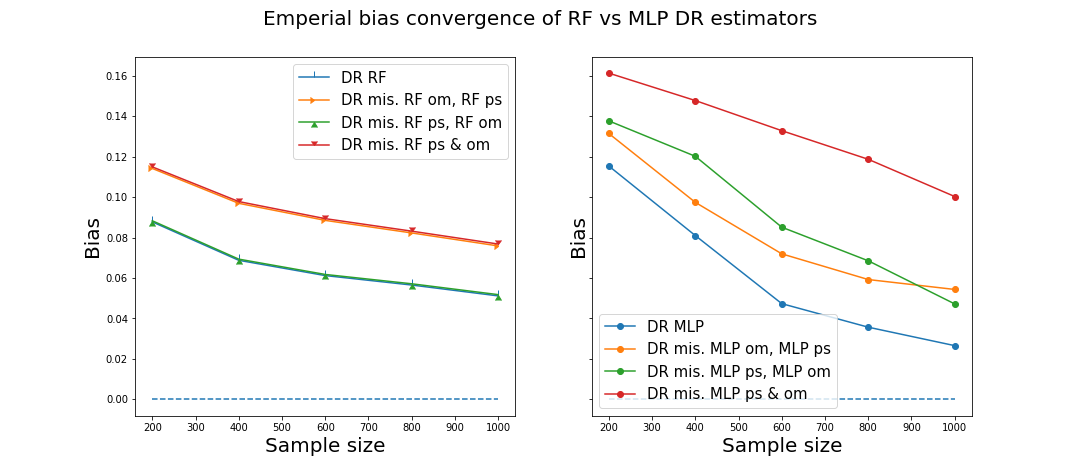
\includegraphics[width = 0.9\columnwidth]{figures/biascompare_moreW.png}
    \caption{Comparing bias performance on simulation with 4 features}
    \label{biascompare_moreW}
\end{figure}

\begin{figure}[h!]
    \centering
    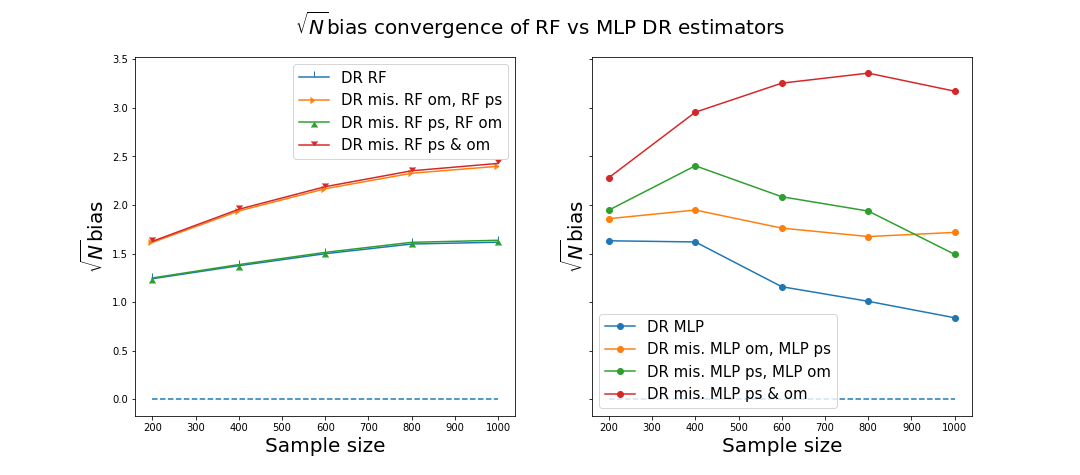
\includegraphics[width = 0.9\columnwidth]{figures/sqrtncompare_moreW.png}
    \caption{Comparing $\sqrt{N}$bias performance on simulations with 4 features}
    \label{sqrtncompare_moreW}
\end{figure}

We had shown in the previous sections that RFs struggled to converge rapidly enough to the true nuisance parameters with the addition of two new features compared to MLPs. We can see this difference in convergence in figures \ref{biascompare_moreW} and \ref{sqrtncompare_moreW}. DR estimators with RFs have a high bias with a rate of convergence slower than that of $N^{-1/2}$. The DR estimators involving MLPs have a high bias that is converging to 0 at a rate faster than that of $N^{-1/2}$, except for the DR estimator with misspecified MLP nuisance parameter models.

\begin{figure}[h!]
    \centering
    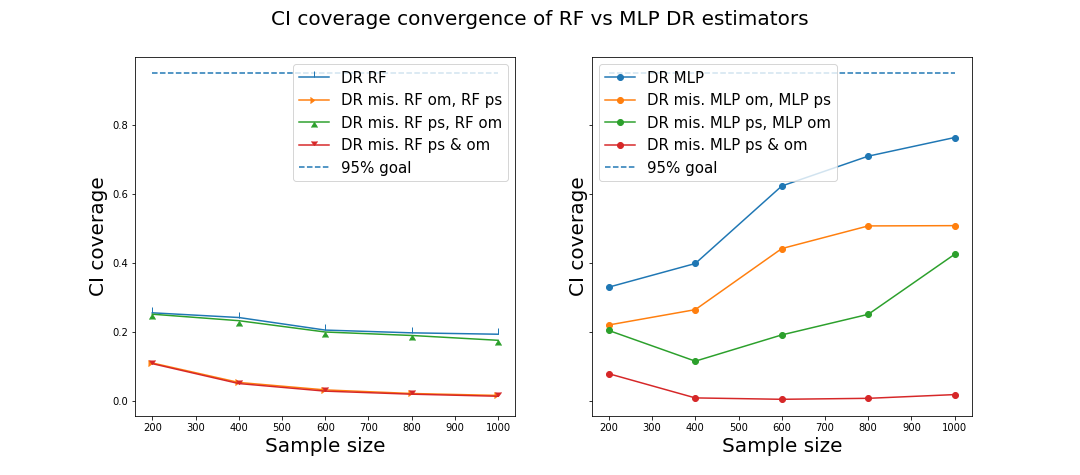
\includegraphics[width = 0.9\columnwidth]{figures/CIcompare_moreW.png}
    \caption{Comparing CI coverage performance for RFs vs MLPs on simulation with 4 features}
    \label{CIcompare_moreW}
\end{figure}

As for CI coverage performance, we can see in figure \ref{CIcompare_moreW} that the DR estimators with RFs fail to reach nominal CI coverage, and the latter is even seeming to converge to 0\%. DR estimators involving at least one correct MLP specification, on the other hand, have CI coverage slowly converging to the 95\% goal.

To summarise, in the 4-feature case, nuisance parameter models based on RFs had a slower convergence rate to the true nuisance parameters compared to MLPs, which resulted in DR estimates with higher bias and poor to nonexistent CI coverage. Models based on MLPs were however not as penalised by the addition of features and provided $N^{-1/2}$-consistent DR estimates with high but converging bias and CIs converging to the nominal coverage, although at a slow rate.

\subsubsection{Limitations}

The main limitation of this study on the use of ML tools in DR estimation is its non-exhaustiveness. Due to time and computational restrictions, we have only looked at 2 data scenarios (2 features vs 4 features defined in previous sections) and two different tools -- RFs and MLPs. With more time and computational power, we would hope that a more exhaustive study of ML tools for DR estimation could be made using different models and data sets. The results we have discussed in sections \ref{2 features} and \ref{4 features} and the comparisons we have made between in RFs and MLPs are not to be taken as generalities. As the name data-adaptive suggests, the power of ML tools comes from being able to adapt to different classification or regression problems on a case by case basis. An ML tool's effectiveness is dependent on the quality of its training data and the tuning of its learning hyperparameters. In theory, we expect these models' predictions to converge to the true values, but in practice, we cannot make general statements on their effectiveness. However, these ML approaches have proven to be efficient at setting nuisance parameter models that converge -- although slowly -- to the true nuisance parameters, when the alternative is a parametric approach that would have likely resulted in misspecification of these models in practice. 

Additionally, throughout the simulations, for each sample size, the ML models were trained and tested then fit on the full data set to be able to compute the DR estimator based on the full data. Hence we might have encountered some over-fitting, which would affect model convergence rates.

Another limitation to note is the range of hyperparameters we have chosen for cross-validations of RFs and MLPs. One would hope to cross-validate on a large range of hyperparameters to finely tune ML tools, but again we were limited by computational power and time. By restricting the cross-validation range we are reducing the chance of picking the hyperparameters that provide the best learning -- and hence convergence -- rate for these models. Our results suggest that in many cases, CIs based on the \cite{lunceford_davidian} SE estimate may not be valid using popular 'off the shelf' implementations of RFs and MLPs, such as small-range cross-validation. Greater care is required in how we tune ML tools to obtain fast learning and convergence rates.

\section{Conclusion}

We hope that this report has provided an insight into the potential of ML tools when used in conjunction with DR estimation. As we have seen throughout the simulations, when the alternative is a parametric approach for setting the nuisance parameter models that are likely to be misspecified in practice, RFs and MLPs provided higher degrees of freedom for getting a correct specification of these models. We have shown some promising results in terms of DR estimator bias convergence rates when using these ML tools. In the simulations we have considered, RFs performed better in terms of DR estimator bias than MLPs, while the latter performed better than the former in a data set with higher dimensions. However, while it is theoretically possible to use ML methods for DR estimation, greater care and research needs to be conducted on which ML tool to choose and how we tune its hyperparameters, to achieve high rates of convergence. Some selection algorithms such as Super Learners and stratified cross-validation exist for model and hyperparameter selection, but we have also shown that CI construction based on the \cite{lunceford_davidian} SE estimation often fail to reach nominal coverage when RFs and MLPs were tuned using simple cross-validation methods. \cite{benkeser2017} have proposed correction methods for recovering nominal CI coverage in nonparametric DR estimation. A more general study on larger sample sizes and different model tuning methods need to be conducted to fully understand the power and potential of ML tools in DR estimation. Although much more time consuming to train than parametric models, if we can streamline model and hyperparameter tuning to achieve higher convergence rates, these ML methods for DR estimation could be the key to further improving the performance and robustness of DR estimators.


%% bibliography
\clearpage
\bibliographystyle{unsrtnat}
\bibliography{bibliography}

\clearpage
\section*{Appendix}
\addcontentsline{toc}{section}{Appendix}

\subsection*{Code for DR simulation}

\lstinputlisting[language=Python]{Code/DR_estimation.py}
\end{document}